\documentclass[a4paper,11pt,norsk,DIV10,twoside,openright,abstracton,idxtotoc,numbers=noenddot]{scrreprt}
\usepackage[latin1]{inputenc}
\usepackage[OT1,T1]{fontenc}
\usepackage{babel}
\usepackage{amsmath}
\usepackage{txfonts}
\usepackage{eurofont}
%% \usepackage{times}
%% \usepackage[subscriptcorrection,slantedGreek,nofontinfo]{mtpro}
%% \usepackage{mtpams}
%% \usepackage{mtpb}
\usepackage{icomma}
\usepackage{soul}
\usepackage[scaled=0.85]{couriers}
\usepackage[squaren]{SIunits}
\usepackage[bottom,symbol,perpage]{footmisc}
\usepackage[center]{caption}
\usepackage{enumitem}
\usepackage{titlesec}
\usepackage{array}
\usepackage{booktabs}
\usepackage{longtable}
\usepackage{ragged2e}
\usepackage{subfig}
\usepackage{listings}
\usepackage{fancyvrb}
\usepackage{upquote}
\usepackage{graphicx}
\usepackage{color}
\usepackage[pdfborder={0 0 0}]{hyperref}
\usepackage{ellipsis}
\usepackage{pdfpages}
\usepackage[expansion=false]{microtype}

%% \onehalfspacing
\frenchspacing

\setlength{\parindent}{\baselineskip}
\setlength{\parskip}{0pt}

\setlength{\fboxrule}{0.5pt}
\setlength{\fboxsep}{0pt}

\addtokomafont{sectioning}{\rmfamily}

\addtokomafont{captionlabel}{\bfseries}

%% \titleformat{\chapter}{\huge\bfseries}{}{}{}[\vspace{0.2\baselineskip}\titlerule]
%% \titlespacing*{\chapter}{0pt}{2.6\baselineskip}{1\baselineskip}

\setcounter{secnumdepth}{4}
\setcounter{tocdepth}{2}

\setcapindent{0em}

%% \renewcommand{\theequation}{\arabic{equation}}

\DefineFNsymbols{stars}[text]{* {**} {***} {****} {*****} {******}}
\setfnsymbol{stars}

\deffootnote[1.5em]{0em}{1.5em}
{\thefootnotemark\hspace{0.1em}}
\deffootnotemark{\thefootnotemark}

\setlist{noitemsep}
\setenumerate{label=\arabic*}
\setitemize[1]{label=\textendash}
\setitemize[2]{label=\ensuremath{\bullet},nolistsep}
\setenumerate[2]{nolistsep}
\setitemize[3]{label=\textendash,nolistsep}
\setenumerate[3]{nolistsep}
\setitemize[4]{label=\ensuremath{\bullet},nolistsep}
\setenumerate[4]{nolistsep}
%% ...

\sloppy

% Alter some LaTeX defaults for better treatment of figures:
% See p.105 of "TeX Unbound" for suggested values.
% See pp. 199-200 of Lamport's "LaTeX" book for details.
%   General parameters, for ALL pages:
\renewcommand{\topfraction}{0.9}	% max fraction of floats at top
\renewcommand{\bottomfraction}{0.8}	% max fraction of floats at bottom
%   Parameters for TEXT pages (not float pages):
\setcounter{topnumber}{2}
\setcounter{bottomnumber}{2}
\setcounter{totalnumber}{4}     % 2 may work better
\setcounter{dbltopnumber}{2}    % for 2-column pages
\renewcommand{\dbltopfraction}{0.9}	% fit big float above 2-col. text
\renewcommand{\textfraction}{0.07}	% allow minimal text w. figs
%   Parameters for FLOAT pages (not text pages):
\renewcommand{\floatpagefraction}{0.7}	% require fuller float pages
% N.B.: floatpagefraction MUST be less than topfraction !!
\renewcommand{\dblfloatpagefraction}{0.7}	% require fuller float pages
% remember to use [htp] or [htpb] for placement

%% Definerer DC-symbolet som Bastian er s� glad i
\newcommand{\Beam}{\raisebox{0.2em}{\includegraphics[width=0.75em]{fig/dc.png}}}

\addtolength{\oddsidemargin}{1cm}
\addtolength{\evensidemargin}{-1cm}

\title{Rapport}
\author{}
\date{}

\begin{document}
\renewcommand{\micro}{\ensuremath{\muup}}
\thispagestyle{empty}

% \begin{titlepage}
%   \newcommand{\HRule}{\rule{\linewidth}{1pt}}

%   \vspace*{\stretch{1}}
%   \noindent\HRule
%   \vspace*{0.5\baselineskip}
%   \begin{center}
%     \Huge
%     \noindent {\bf Virtuell arm\\
%       for funksjonshemmede}\\[1.25\baselineskip]
%     \large
%     % \noindent\emph{Logo (HiST)}
%     \noindent\large\caps{Stian~Rishaug, Bastian~S.~Solem,}\\
%     \noindent\large\caps{Aleksander~Uthus~og~Vegard~�ye}\\[\baselineskip]

%     \noindent Veileder: Herman Ranes

%   \end{center}
%   \vspace*{0.5\baselineskip}
%   \noindent\HRule
%   \vspace*{\stretch{0.75}}
%   \begin{center}
%     
\includegraphics[width=6.5cm]{fig/hist-logo}\\[\baselineskip]
%     \vspace*{0.25\baselineskip}

%     \noindent {\large Trondheim, mai 2009}
%   \end{center}
% \end{titlepage}

\begin{titlepage}
\includepdf{fig/forside.pdf}
\end{titlepage}

\addcontentsline{toc}{chapter}{Sammendrag}

\begin{abstract}
  \noindent P� oppdrag fra SINTEF er det laget en prototype til en
  \emph{tungestyrt musepeker} som kan brukes p� Microsoft Windows via standard
  HID-musegrensesnitt. Musepekeren aktiveres av forspente trykkf�lsomme
  resistanser av typen FSR-400 og FSR-402. Disse sensorene er sv�rt f�lsomme,
  og har en hysteresefunksjon ved kontinuerlig trykk. Det er derfor laget
  en automatisk kalibreringsrutine som bruker av musen kan aktivere manuelt i
  tilfellet musepekeren oppf�rer seg u�nsket.

  For plassering av sensorene er det laget en justerbar \emph{hodeb�yle}.
  Hodeb�ylen er bygd av et noe svakt material, og m�ten sensorene er festet p�,
  b�r forskes videre p�. Ved videreutvikling av den valgte designen kan
  hodeb�ylen bli meget bra.

  Elektronikken som behandler data og <<styrer>> musepekeren, er demokretsen
  \emph{AT90USBKey} fra Atmel. Kretsen har innebygde ADC-er, som benyttes til
  tolking av sensordata. Den gj�r bruk av USB-grensesnittet for overf�ring av
  data, s� vel som energitilf�rsel. Det er integrert en spenningsregulator som
  benyttes til � forspenne sensorene. Regulatoren er sterk nok til � forsyne
  eventuelle tilleggskretser.

  Programkoden er skrevet for � v�re fleksibel ang�ende antall sensorer og
  portene de kobles til, s� vel som valg av mikrokontroller. Programkoden
  foreligger som vedlegg til rapporten.

  Bruk av musen fungerer slik: Brukeren starter en bevegelse og stopper eller
  endrer retning ved �nsket plassering. Pekeren seg langsomt til � begynne med
  for � gi god presisjon. Man kan snakke mens man beveger musepekeren over
  skjermen, og det er mulig � be venstre museknapp v�re aktiv mens man beveger
  musepekeren over skjermen. Det er ogs� mulig � sette musen i en
  <<scroll>>-modus som gj�r surfing av nettsider og lesing av dokumenter meget
  behagelig.

  Utgiftene ved prosjektet var minimale, estimert til ca. 2000 NOK.\\

  \noindent P� bakgrunn av rapporten konkluderer prosjektgruppen med at
  \emph{det er mulig � lage en tungestyrt musepeker med de valgte sensorene}.
  Det mekaniske og ergonomiske m� imidlertid forbedres for � f� et salgbart
  produkt.
\end{abstract}


\addcontentsline{toc}{chapter}{Forord}
\chapter*{Forord}

Rapporten er en avsluttende bacheloroppgave i elektro- og datateknikk:
fordypning i elektronikk ved H�yskolen i S�r-Tr�ndelag. Oppgaven er definert i
sammarbeid med SINTEF og veileder Herman Ranes fra HiST. Arbeidet er utf�rt i
HiST sine lokaler og har hatt en varighet fra 26. januar 2009 frem til 25. mai
2009. Rapporten er et resultat av dr�ye 4 m�neders forskning og uttesting av en
prototype for for en tungestyrt datamus som kan brukes i Microsoft Windows.
Bakgrunnen for oppgaven er � gi en konklusjon til SINTEF, om det er mulig bruke
trykkresistive f�lere av typen FSR-400 og FSR-402 for dette form�let. Det er
�nsket � kunne gi et svar p� om denne teknologien er tilstrekkelig for � gi en
l�sning p� problemstillingen.

\begin{center}
  \noindent \textbf{\large Vi vil i denne anledning rette en takk til}
\end{center}
\vspace*{-\baselineskip}
\begin{center}
  \emph{Ansatte ved HiST}
\end{center}
\vspace*{-1.5\baselineskip}
\begin{center}
  Herman Ranes

  Rolf Kristian Snilsberg
\end{center}
\vspace*{-\baselineskip}
\begin{center}
  \emph{Personer med tilknytning til rapporten}
\end{center}
\vspace*{-1.5\baselineskip}
\begin{center}
  Tone Berg

  Mats Ekstr�m
\end{center}

\vspace*{5\baselineskip}
Trondheim, 24. mai 2009


\tableofcontents

\chapter{Innledning}

\begin{quote}\it
  \textbf{Sammendrag:} Resultatet av prosjektet skal bli en prototype for
  tungestyrt musepeker som kan brukes p� Microsoft Windows. Denne prototypen
  skal lages med trykkf�lsomme resistanser. Ettersom det ikke finnes noe
  tilsvarende produkt p� det norske markedet, kan et vellykket produkt dekke et
  viktig behov for funksjonshemmede som er ute av stand til � bruke en h�ndstyrt
  datamus.
\end{quote}

\section{Bakgrunn/tidligere l�sninger} % kort!

Bacheloroppgave p� oppdrag fra SINTEF: Det skal bygges et verkt�y for
funksjonshemmede som lar datamusen styres med tungen. Prosjektet fokuserer p� �
kartlegge hvor godt ideen med tungesensorer fungerer i praksis. Overfor
oppdragsgiver er det \emph{to�rig taushetsplikt}, siden oppdragsgiver �nsker �
kunne bruke resultatene av prosjektet til egne form�l. Prosjektgruppen best�r av
fire studenter p� tredje �ret bachelor i elektro- og datateknikk: fordypning i
elektronikk ved H�yskolen i S�r-Tr�ndelag. Ved tidligere prosjekter er det gjort
fors�k med:
\begin{itemize}
\item Induktive f�lere (reagerer p� metall og er billige i innkj�p)
\item Touch (en form for kapasitiv f�ler)
\item IR (Vanskelig metode for avlesning)
\item Kapasitive f�lere (sv�rt dyre i innkj�p)
\end{itemize}
Det er �nskelig at gruppen starter prosjektet fra <<scratch>>, for � se om
resultatet benytter seg av alternative metoder til dem som er brukt tidligere.

\section{Problemstilling}
\label{sec:hovedproblemstilling}

Ved endt prosjekt skal det legges frem en prototype som kan styre musepekeren i
Microsoft Windows ved bruk av tungen, og som har de samme mulighetene som en
ordin�r mus. Prosjektgruppen har f�tt utdelt trykksensorer (FSR-400 og FSR-402),
produsert av Interlink Electronics (sensorene kapittel~\ref{sec:sensorkap}).
Prosjektet skal kunne svare p� om sensorene kan brukes til et ferdig produkt.
Det skal kommes frem til en konfigurasjon av sensorplassering, og algoritmer for
behandling av sensordata.

\subsection{Hva skal gj�res og hvordan}

\begin{itemize}
  % tekts sensortesting h�r vegard (egentlig til bastian, men skriver vegard for
  % god s�knings venlighet,)
\item Kartlegge hvordan de utdelte sensorene kan brukes
  (kap.~\ref{sec:sensorkap}).
\item Det skal lages en hodeb�yle for enkel bruk av datamusen
  (kap.~\ref{sec:hodeboyle}).
\item Det skal lages en krets for signalbehandling, fortrinnsvis en
  mikrokontroller med ADC (kap.~\ref{sec:elektronikk}).
\item Overf�ringsgrensesnitt mot Microsoft Windows -- Bluetooth/USB
  (kap.~\ref{sec:elektronikk}).
\item Det skal tas standpunkt til hvor prosesseringen av data skal foreg�, f�r
  eller etter signalet har kommet til datamaskinen (kap.~\ref{sec:elektronikk}).
\item Valg av sensorkonfigurasjon, antall og plassering, brukergrensesnitt
  (kap.~\ref{sec:funksjonalitet}).
\item Program for tolkning av avlest sensordata m� skrives
  (kap.~\ref{sec:funksjonalitet}).
\end{itemize}

\subsection{Overordnet spesifikasjon av konseptet}
\label{sec:produktspes}

Bruken av funksjonene er beskrevet i kapittel~\ref{sec:funksjonalitet}, som tar
for seg funksjonalitet og brukergrensesnitt. Konseptet skal inneholde disse
standard musefunksjonene:
\begin{itemize}
\item Bevegelse
  \begin{itemize}
  \item Horisontal
  \item Vertikal
  \item Diagonalt
  \item 3 Hastigheter
  \end{itemize}
\item Knapper
  \begin{itemize}
  \item Venstre museknapp
  \item H�yre museknapp
  \item Scroll
  \end{itemize}
\end{itemize}
Festemekanismen beskrevet i kapittel~\ref{sec:hodeboyle} er en hodeb�yle med
disse spesifikasjonene:
\begin{itemize}
\item Behagelig � bruke, ogs� over lengre tid (viktig at det ikke er for tungt).
\item Uproblematisk � ta utstyret av/p� for en person som skal hjelpe brukeren.
\item Tilpassningsmulighet for flere brukere uansett hodest�rrelse/form.
\item Det skal v�re et godt press p� sensorene mot kinnet, slik at det er lett �
  bruke musen.
\end{itemize}
For hodeb�ylen er utseendemessig design nedprioritert. Av funksjoner er ingen
valgt bort.


\cleardoublepage

\chapter[Sensorene (Solem og �ye)]{Sensorene}
\label{sec:sensorkap}

\begin{quote}\it
  \textbf{Sammendrag:} Tar for seg forspenningskretsen i teori og praksis.
  Teorien tilsier at sensorene b�r forspennes med en motstand p�
  8--15~$\mathit{k\Omega}$. M�lingene viser hvordan sensorene oppf�rer seg under
  ulike omstendigheter. Sensorkarakteristikken setter krav til en dynamisk verdi
  for hendelsesaktivering, og kontinuerlig kalibrering. % konklusjon
\end{quote}

\section{Teori: forspenning av trykksensorene}

%% \newcommand*{\appropto}{\mathrel{\vcenter{\offinterlineskip\vskip0.4ex\hbox{$\propto$}\hbox{$\sim$}}}}

\begin{figure}[h]
  \centering
  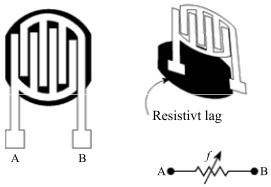
\includegraphics[height=5cm]{fig/trykksensor.pdf}
  \caption{Resistive trykksensorer}
  \label{fig:trykksensorer}
\end{figure}

\noindent Sensorene som brukes, er \emph{resistive trykksensorer}
(fig.~\ref{fig:trykksensorer}), eller trykkf�lsomme motstander. De best�r av av
to deler: polymerbasert tykkfilm koblet til et resistivt materiale, og
polymerbasert tykkfilm koblet til elektroniske kontakter. Polymer er en type
bindingsmiddel som brukes p� motstander og ledere. N�r dette presses sammen, gir
det �kt konduktivitans (lederevne) gjennom kretsen~\cite{interlink}.

Dermed fungerer sensorene som en variabel motstand under trykk (jo h�yere trykk,
jo lavere resistans), og som et brudd (uendelig resistans) ellers.

\begin{figure}[t]
  \centering
  \subfloat[]{\label{fig:litensensor}\includegraphics[clip=true,height=6cm,page=11,trim={120
      400 400 140}]{fig/fsrguide.pdf}}\qquad\qquad
  \subfloat[]{\label{fig:storsensor}\includegraphics[clip=true,height=6cm,page=11,trim={375
      400 135 140}]{fig/fsrguide.pdf}}
  \caption[Sensortyper, FSR-400 og FSR-402]{Sensor type FSR-400~\subref{fig:litensensor},
    sensor type FSR-402~\subref{fig:storsensor}.\\
    Millimeterm�l er gitt i klammer.}
  \label{fig:sensortyper}
\end{figure}

Sensorene, som produseres av Interlink Electronics,\footnote{Nettside:
  \url{http://www.interlinkelectronics.com/}.} kommer i to typer
(fig.~\ref{fig:sensortyper}): \subref{fig:litensensor} en \emph{liten} sensor
med en diameter p� 8~mm (FSR-400), og \subref{fig:storsensor} en \emph{stor}
sensor p� 18~mm (FSR-402). Det trykkf�lsomme omr�det er litt mindre og er p�
hhv. 5~mm og 14~mm.

\begin{figure}[b]
  \centering
  \subfloat[]{\label{fig:forspenning}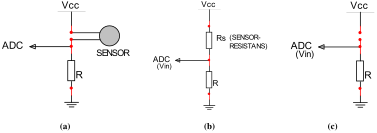
\includegraphics[height=4.2cm]{fig/sensor.pdf}}
  \qquad
  \subfloat[]{\label{fig:spenningsdeling}\includegraphics[height=4.2cm]{fig/spenningsdeling.pdf}}
  \qquad
  \subfloat[]{\label{fig:brudd}\includegraphics[height=4.2cm]{fig/brudd.pdf}}
  \caption[Forspenning av trykksensor, spenningsdeling og brudd]{Forspenning av
    trykksensor~\subref{fig:forspenning},
    spenningsdeling~\subref{fig:spenningsdeling} og brudd~\subref{fig:brudd}}
  \label{fig:sensor}
\end{figure}

For � f� m�lbare trykkverdier, m� sensorene \emph{forspennes}
(fig.~\ref{fig:forspenning}). Hver sensor kobles i serie med en motstand $R$,
som g�r til jord. I den andre enden p�trykkes en tilf�rselsspenning $V_{CC}$ p�
3,3~V. Dette oppsettet gir en spenningsdeling mellom sensorresistansen, $R_S$,
og $R$:
\begin{equation}
  \label{eq:spenningsdeling}
  V_{IN} = V_{CC} \cdot \frac{R}{R_S + R}
\end{equation}
$V_{IN}$ sendes inn p� analog-til-digital-omformeren p� kortet (ADC-en), og er
alts� verdien som programmet p� mikrokontrolleren <<ser>>. Gjennom ADC-en f�r vi
en overgang fra den \emph{fysiske} st�rrelsen $V_{IN}$ til den \emph{digitale}
8-bit verdien \texttt{\textit{ADC\_VARIABEL}} i programkoden:
\begin{equation}
  \label{eq:datablad}
  \text{\texttt{\textit{ADC\_VARIABEL}}}
  = \frac{V_{IN} \cdot 255}{V_{REF}}
\end{equation}
$V_{REF}$ er \emph{referansespenningen} og er lik $V_{CC}$. Den maksimale
verdien for \texttt{\textit{ADC\_VARIABEL}}, 255, svarer dermed til 3,3~V, og
\texttt{\textit{ADC\_VARIABEL}} er proporsjonal med $V_{IN}$.

For � velge en passende verdi for forspenningsmotstanden $R$, m� vi se hvordan
den p�virker forholdet mellom trykk og spenning. Dette forholdet kan brytes opp
i to mindre: forholdet mellom trykk~($\rho$) og sensorresistans~($R_S$), og
forholdet mellom sensorresistans~($R_S$) og m�lt spenning~($V_{IN}$).

M�linger p� $\rho$--$R_S$-forholdet er gitt i avsnitt~\ref{sec:malinger}, og kan
i korte trekk oppsummeres slik: for lette trykk er $R_S \approx 100$~\kilo\ohm,
og for harde trykk g�r $R_S$ ned til 20~\kilo\ohm, med sterkt avtagende stigning
(fig.~\ref{fig:litenok}, s.~\pageref{fig:litenok}). Forholdet er alts� sterkt
uline�rt: $R_S$ er stor n�r $\rho$ er liten, og $R_S$ er liten n�r $\rho$ er
stor.

Det samme gjelder for $R_S$--$V_{IN}$-forholdet, gitt i
ligning~(\ref{eq:spenningsdeling}): n�r den ene g�r opp, g�r den andre ned.
Summen av disse to <<inverse>> forholdene er at $\rho$ og $V_{IN}$ �ker i takt:
n�r trykket �ker, s� �ker den m�lte spenningen, og n�r trykket minker, s� minker
spenningen. N�r $\rho = 0$, s� er ogs� $V_{IN} = 0$, og i programkoden har
\texttt{\textit{ADC\_VARIABEL}} verdien 0. Dette er det ideelle
\emph{nullniv�et}, verdien n�r sensoren ikke er i bruk. \label{sec:nullnivaa}

% \begin{displaymath}
%   R_S \overset{\text{tiln.}}{\propto} \frac{1}{\rho}
% \end{displaymath}
% der $\overset{\text{tiln.}}{\propto}$ betyr <<tiln�rmet proporsjonal med>>.
% Sensorresistansen kan dermed, \emph{i upresise termer}, betraktes som en slags
% <<invers>> av trykket: $R_S$ er stor n�r $\rho$ er liten, og $R_S$ er liten
% n�r $\rho$ er stor. Tilsvarende kan den m�lte spenningen, $V_{IN}$, betraktes
% som <<inversen>> av $R_S$:
% \begin{displaymath}
%   V_{IN} \overset{\text{tiln.}}{\propto} \frac{1}{R_S}
% \end{displaymath}
% Dette er en forenklet m�te � uttrykke innholdet i
% ligning~(\ref{eq:spenningsdeling}) p�.\footnote{Dersom $R$ holdes konstant, er
%   den matematiske beskrivelsen av $R_S$--$V_{IN}$-kurven at den antar
%   \emph{hyperbolsk vekst}.} Legger vi sammen disse forenklingene, f�r vi at
% \begin{displaymath}
%   V_{IN} \overset{\text{tiln.}}{\propto} \rho
% \end{displaymath}
% Dvs. den m�lte spenningen, $V_{IN}$ (alias \texttt{\textit{ADC\_VARIABEL}} i
% programkoden), er \emph{tiln�rmet proporsjonal} med trykket, $\rho$.

\begin{figure}
  \centering
  \subfloat[]{\label{fig:vin3d}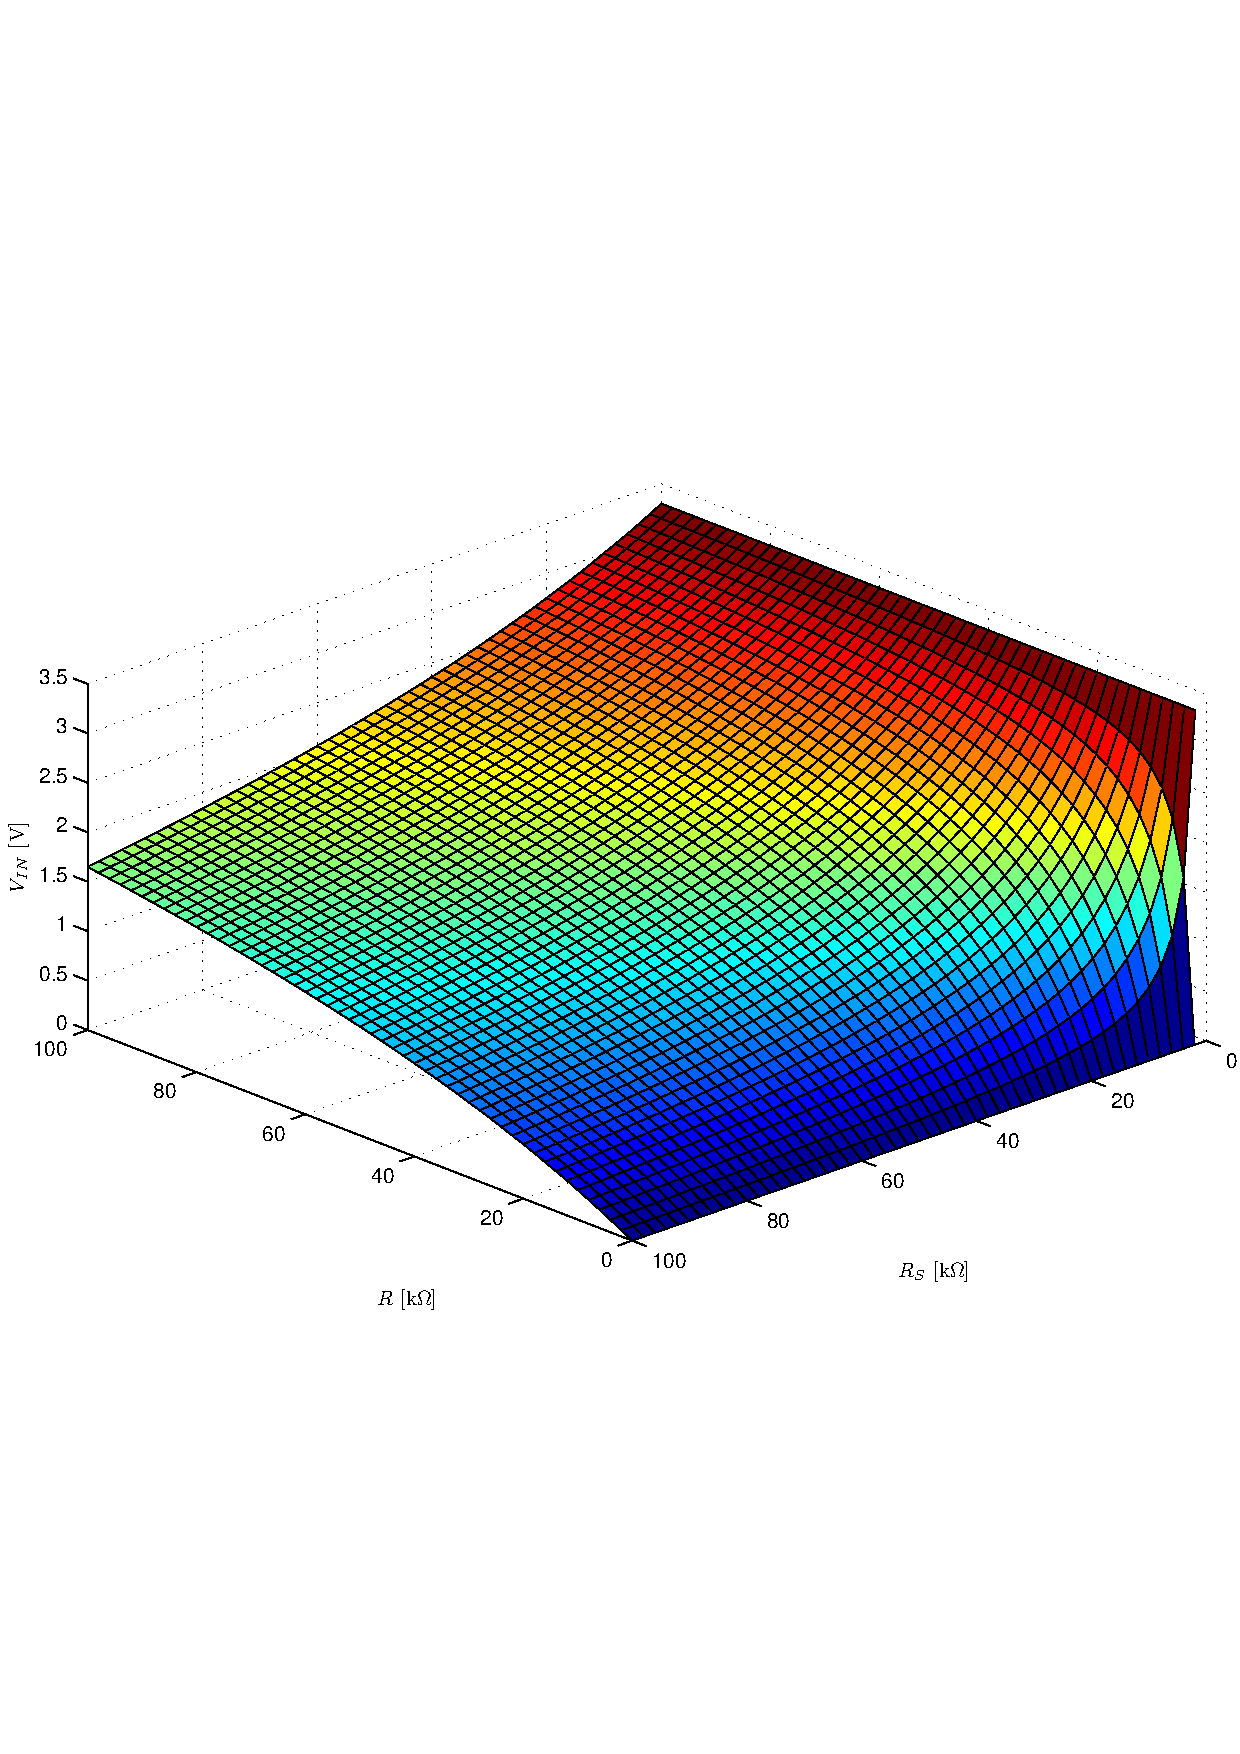
\includegraphics[height=4.7cm]{fig/vin3d.pdf}}\quad
  \subfloat[]{\label{fig:vin2d}\includegraphics[height=4.7cm]{fig/vin2d.pdf}}
  \caption[Spenning som funksjon av sensorresistans og motstand]{$V_{IN}$ som
    funksjon av $R$ og $R_S$, ligning~(\ref{eq:spenningsdeling})}
  \label{fig:vin}
\end{figure}

% \begin{figure}
%   \centering
%   \subfloat[]{\label{fig:partvin3d}\includegraphics[height=5cm]{fig/partvin3d.pdf}}
%   \subfloat[]{\label{fig:partvin2d}\includegraphics[height=5cm,clip=true,trim={0
%       0 0 10}]{fig/partvin2d.pdf}}
%   \caption[Den partiellderiverte av spenningen mht. sensorresistans]{Plott av
%     den partiellderiverte av $V_{IN}$ med hensyn til $R_S$,
%     ligning~(\ref{eq:partiell})}
%   \label{fig:partvin}
% \end{figure}

Hvis 0~V er spenningen som m�les for intet trykk, hva er da spenningen for et
lett trykk (n�r $R_S = 100$~\kilo\ohm)? Det er viktig at denne verdien ikke er
for lav, ellers vil den ikke reliabelt kunne skilles fra nullniv�et:
$V_{IN\,\text{min}} > 0$~V. Figur \ref{fig:vin} viser hvordan
forspenningsmotstanden $R$ innvirker p� forholdet mellom $R_S$ og $V_{IN}$. N�r
sensoren tas i bruk, vil vi f� et \emph{sprang} p� minst minimumsverdien,
$V_{IN\,\text{min}}$, som selvf�lgelig ikke b�r v�re s� lav at spranget ikke
registreres. Men den b�r heller ikke v�re for h�y, ellers f�r vi ikke utnyttet
intervallet av $V_{IN}$-verdier (verdiomr�det) skikkelig.

Vi ser ogs� at sammenhengen mellom $R_S$ og $V_{IN}$ blir \emph{mer uline�r} for
lavere verdier av $R$. Ulinearitet er ikke n�dvendigvis negativt. Si at vi
�nsker at pekerfarten skal v�re konstant for lette trykk ($R_S =
\text{40--100}$~\kilo\ohm), men at den skal �ke for harde trykk ($R_S <
40$~\kilo\ohm). Da er det gunstig med \emph{lav oppl�sning} for <<lette trykk>>
og \emph{h�y oppl�sning} for <<harde trykk>>. Det vil si at vi bruker en st�rre
del av intervallet av $V_{IN}$-verdier til � differensiere mellom de <<harde
trykkene>>, mens de <<lette trykkene>> delegeres til et snevrere utsnitt.

Veier vi disse hensynene opp mot hverandre, ser vi at en motstand p�
8--15~\kilo\ohm\ kan v�re egnet. Dette gir $V_{IN\,\text{min}} =
\text{0,24--0,43}$~V, som svarer til $\text{\texttt{\textit{ADC\_VARIABEL}}} =
\text{19--33}$: godt over det ideelle nullniv�et, og god utnyttelse av
verdiomr�det.

Men hvordan fungerer sensorene i praksis? Endres sensorresistansen over tid? Er
nullniv�et alltid 0~V? For � f� svar p� disse sp�rsm�lene, m� vi foreta noen
m�linger.

\section{M�linger}

\label{sec:malinger}

\noindent For � fastsl� hvordan sensorene oppf�rer seg under ulike
omstendigheter, er det foretatt tre forskjellige typer m�linger p� sensorene.
Denne informasjonen er n�dvendig for � avgj�re sensorenes muligheter og
begrensninger. Utstyret som er benyttet for disse m�lingene er gitt i
tabell~\ref{tab:utstyrliste}.

\begin{table}[h]
  \centering
  \caption[Utstyrsliste for m�linger p� sensorer]{Utstyrsliste}
  \begin{tabular}{ll}
    \toprule
    Instrument/maskin  & Type/data\\
    \midrule
    Motstand           & 8,2~\kilo\ohm\\
    Spenningsforsyning & 4,5~V\Beam\\ % DC
    Vektenhet          & 4,35~g (kronestykke)\\
    Vektarm            & 18~g\\
    Multimeter         & \\
    \bottomrule
  \end{tabular}
  \label{tab:utstyrliste}
\end{table}

\noindent For � �ve et konstant trykk p� sensorene, er det brukt en arm som det
blir lagt vektenheter p�, figur~\ref{fig:malepinne}. Hvor p� sensorens overflate
trykket settes, innvirker p� motstandsverdien, men armen s�rger for � holde
kontaktflaten og trykkomr�det tiln�rmet konstant, figur~\ref{fig:sensorpress}.
Uten vektenheter veier armen 18~g.

\subsection[Motstandsverdi ved varierende trykk]{Motstandsverdi ved varierende
  trykk FSR-400}
\label{sec:litenvar}
Motstandsverdien til $R_S$ (i \kilo\ohm) m�les som direkte f�lge av trykk p�
overflaten til en sensor av typen FSR-400 (\textit{liten sensor}). M�lingene
foretas med 5~s mellomrom. Hensikten med denne m�lingen er � se hvordan et
konstant trykk p�virker $R_S$ over tid og hva som skjer n�r trykket minker. G�r
$R_S$-verdien tilbake til utgangspunktet, eller er den endret som f�lge av at
sensoren har v�rt i bruk? Dette er et viktig sp�rsm�l hva nullniv�et ang�r
(tidligere omtalt p� s.~\pageref{sec:nullnivaa}).

M�leresultatene er gitt i tabell~\ref{tab:litenvar} og
figur~\ref{fig:litenvar}.

\subsubsection{Dr�fting av resultatene}

Som man kan se av tabell~\ref{tab:litenvar} er resistansen i sensoren ved 26,7~g
(tilstand~0) lik uendelig -- sensoren leder ikke. N�r trykket s� �ker til
31,05~g (tilstand~1), leder sensoren. Deretter lar man sensoren v�re i
tilstand~1 i 20~s, og observerer at resistansen minker, se
figur~\ref{fig:litenvar}. Men n�r man n� g�r tilbake til tilstand~0, kan man se
at sensoren \emph{fortsatt leder}.

Sensorresistansen har alts� en slags \emph{hysteresefunksjon}. Over tid vil
denne hysteresen �ke noe. Dette m� det tas h�yde for n�r sensorene skal avleses:
Man kan ikke sammenligne de avleste verdiene med et fastsatt nullniv� p� 0~V,
men m� i stedet s�rge for � \emph{kalibrere} nullniv�et med jevne mellomrom.

\begin{table}[tpb]
  \centering
  \caption{Liten sensor, varierende vekt}
  \begin{tabular}{llll}
    \toprule
    Vektenheter [stk.] &
    Tillegg til arm [g] &
    Total vekt [g] &
    $R_S$ [\kilo\ohm]\\
    \midrule
    0 & 0,00  & 18,00 & --\\
    2 & 8,70  & 26,70 & --\\
    3 & 13,05 & 31,05 & 111\\
    3 & 13,05 & 31,05 & 97\\
    3 & 13,05 & 31,05 & 93\\
    3 & 13,05 & 31,05 & 70\\
    2 & 8,70  & 26,70 & 120\\
    3 & 13,05 & 31,05 & 74\\
    2 & 8,70  & 26,70 & 108\\
    3 & 13,05 & 31,05 & 71\\
    3 & 13,05 & 31,05 & 69\\
    3 & 13,05 & 31,05 & 66\\
    2 & 8,70  & 26,70 & 87\\
    \bottomrule
  \end{tabular}
  \label{tab:litenvar}
\end{table}

\begin{figure}[tpb]
  \centering
  \includegraphics[clip=true,page=2,trim={80 265 145
    390},width=0.9\linewidth]{fig/sensormalinger.pdf}
  \caption[Liten sensor, varierende vekt]{Liten sensor, varierende vekt
    (tabell~\ref{tab:litenvar})}
  \label{fig:litenvar}
\end{figure}

\clearpage

\subsection[Spenningsverdi ved �kende trykk, vektene av]{Spenningsverdi ved
  �kende trykk, vektene av mellom hver m�ling}

\label{sec:okav}

\noindent Sensorene blir koblet opp som i figur~\ref{fig:sensor} og spenningen
over $R$ blir m�lt ved trykk p� sensoren. Mellom hver m�ling tas vektene av, og
trykket blir 18~g.\footnote{Lar m�learmen ligge for � holde trykkomr�det
  konstant. Vekten p� armen er s� liten at sensorene p�virkes minimalt av denne,
  se kapittel~\ref{sec:litenvar}} M�lingene foretas 5~s etter at vekten er lagt
p�. Spenningen som m�les er spenningen ADC-en p� kortet ser, s� hensikten er �
m�le hvordan spenningen stiger ved enkelttrykk.

For m�lingene gjelder ligning~(\ref{eq:spenningsdeling}),
s.~\pageref{eq:spenningsdeling}, samt sammenhengene
\begin{align}
  R_S &= \frac{V_{CC} - V_R}{I_R}\label{eq:resistans}\\
  I_R &= \frac{U_R}{R}\label{eq:strom}
\end{align}
M�lingene er foretatt med $V_{CC} = 4,5$~V og $R = 8,2$~\kilo\ohm. Valget av
verdier er basert p� utstyret som var tilgjengelig da m�lingene ble foretatt.

Resultatene for \textit{liten sensor} (FSR-400) er gitt i
tabell~\ref{tab:litenokav} og figur~\ref{fig:litenokav}, og resultatene for
\textit{stor sensor} (FSR-402) er gitt i tabell~\ref{tab:storokav} og
figur~\ref{fig:storokav}.

\subsubsection{Dr�fting av resultatene}

Av figur~\ref{fig:litenokav} og \ref{fig:storok}, som viser spenning og motstand
mot trykk for hhv. liten og stor sensor, kan man se at de to typene gir ganske
like resultater. Den store sensoren har en noe brattere kurve. Dette kan komme
av den st�rre overflaten, og at buen p� overflatemembranen minker resistansen
over et st�rre omr�de enn det som faktisk er i kontakt med armen, illustrert i
figur~\ref{fig:sensorpress}.

Det kommer frem av resultatene i figur~\ref{fig:litenokavspenning} og
figur~\ref{fig:storokavspenning} at spenningens stigningsendring er ganske jevnt
fordelt over trykkomr�det. Det er derimot ikke den fallende endringen til
sensorverdien som man kan se i figur~\ref{fig:litenokavmotstand} og
figur~\ref{fig:storokavmotstand}. Dette skyldes den uline�re sammenhengen i
ligning~(\ref{eq:spenningsdeling}).

Spenningsstigningen har noen ujevnheter, dette kan v�re fordi kontaktpunktet har
en un�yaktighet p� $\pm 1$~mm n�r vektene tas av.

\begin{figure}[b]
  \centering
  \includegraphics[width=0.5\linewidth]{fig/malepinne.png}
  \caption[Arm for sensorm�linger]{Arm for � legge vekt(er) p� sensorene}
  \label{fig:malepinne}
\end{figure}

\begin{figure}[b]
  \centering
  \includegraphics[width=0.4\linewidth]{fig/sensorpress.png}
  \caption{Sensor under trykk}
  \label{fig:sensorpress}
\end{figure}

\clearpage

\begin{table}[t]
  \centering
  \caption[Liten sensor, �kende vekt, vektene av]{Liten sensor, �kende vekt, vektene av mellom hver m�ling}
  \begin{tabular}{lllll}
    \toprule
    $V_R$ [V] &
    Vekt [g] &
    Vektenheter [stk.] &
    Utr. $I_R$ [\micro\ampere] &
    Utr. $R_S$ [\kilo\ohm]\\
    \midrule
    0,20 & 18,00 & 0  & 24,39  & 176,30\\
    0,38 & 22,35 & 1  & 46,34  & 88,91\\
    0,72 & 26,70 & 2  & 87,80  & 43,05\\
    1,02 & 31,05 & 3  & 124,39 & 27,98\\
    1,13 & 35,40 & 4  & 137,80 & 24,45\\
    1,28 & 39,75 & 5  & 156,10 & 20,63\\
    1,29 & 44,10 & 6  & 157,32 & 20,40\\
    1,56 & 48,45 & 7  & 190,24 & 15,45\\
    1,60 & 52,80 & 8  & 195,12 & 14,86\\
    1,70 & 57,15 & 9  & 207,32 & 13,51\\
    1,67 & 61,50 & 10 & 203,66 & 13,90\\
    1,75 & 65,85 & 11 & 213,41 & 12,89\\
    1,90 & 70,20 & 12 & 231,71 & 11,22\\
    1,96 & 74,55 & 13 & 239,02 & 10,63\\
    2,01 & 78,90 & 14 & 245,12 & 10,16\\
    2,07 & 83,25 & 15 & 252,44 & 9,63\\
    2,12 & 87,60 & 16 & 258,54 & 9,21\\
    2,18 & 91,95 & 17 & 265,85 & 8,73\\
    2,20 & 96,30 & 18 & 268,29 & 8,57\\
    \bottomrule
  \end{tabular}
  \label{tab:litenokav}
\end{table}

\begin{table}[b]
  \centering
  \caption[Stor sensor, �kende vekt, vektene av]{Stor sensor, �kende vekt, vektene av mellom hver m�ling}
  \begin{tabular}{lllll}
    \toprule
    $V_R$ [V] &
    Vekt [g] &
    Vektenheter [stk.] &
    Utr. $I_R$ [\micro\ampere] &
    Utr. $R_S$ [\kilo\ohm]\\
    \midrule
    0,27 & 18,00 & 0  & 32,93  & 128,47\\
    0,63 & 22,35 & 1  & 76,83  & 50,37\\
    0,96 & 26,70 & 2  & 117,07 & 30,24\\
    1,25 & 31,05 & 3  & 152,44 & 21,32\\
    1,35 & 35,40 & 4  & 164,63 & 19,13\\
    1,54 & 39,75 & 5  & 187,80 & 15,76\\
    1,65 & 44,10 & 6  & 201,22 & 14,16\\
    1,65 & 48,45 & 7  & 201,22 & 14,16\\
    1,67 & 52,80 & 8  & 203,66 & 13,90\\
    1,80 & 57,15 & 9  & 219,51 & 12,30\\
    1,90 & 61,50 & 10 & 231,71 & 11,22\\
    1,94 & 65,85 & 11 & 236,59 & 10,82\\
    2,08 & 70,20 & 12 & 253,66 & 9,54\\
    \bottomrule
  \end{tabular}
  \label{tab:storokav}
\end{table}

\clearpage

\begin{figure}[t]
  \centering \subfloat[Spenning mot
  trykk]{\label{fig:litenokavspenning}\includegraphics[clip=true,page=4,trim={80
      490 145 115}]{fig/sensormalinger.pdf}}

  \subfloat[Motstand mot trykk, utregnet fra
  \subref{fig:litenokavspenning}]{\label{fig:litenokavmotstand}\includegraphics[clip=true,page=4,trim={80
      190 145 410}]{fig/sensormalinger.pdf}}

  \caption[Liten sensor, �kende vekt, vektene av]{Liten sensor, �kende vekt,
    vektene av mellom hver m�ling (tabell~\ref{tab:litenokav})}
  \label{fig:litenokav}
\end{figure}

\begin{figure}[b]
  \centering \subfloat[Spenning mot
  trykk]{\label{fig:storokavspenning}\includegraphics[clip=true,page=8,trim={80
      490 275 110}]{fig/sensormalinger.pdf}}

  \subfloat[Motstand mot trykk, utregnet fra
  \subref{fig:storokavspenning}]{\label{fig:storokavmotstand}\includegraphics[clip=true,page=8,trim={80
      190 150 410}]{fig/sensormalinger.pdf}}

  \caption[Stor sensor, �kende vekt, vektene av]{Stor sensor, �kende vekt,
    vektene av mellom hver m�ling (tabell~\ref{tab:storokav})}
  \label{fig:storokav}
\end{figure}

\clearpage

\subsection{Spenningsverdi ved �kende trykk, vektene ikke av}

Som tidligere i avsnitt~\ref{sec:okav} m�les spenningen over $R$, men vektene
blir n� \emph{ikke} tatt av mellom hver m�ling. Dette er for � minske muligheten
for bevegelse p� armen, og for � vise forventet spenning/spenningsendring i
tilfelle konstant trykk p� sensoren. Her venter man 15~s mellom m�lingene for �
la verdien bli tiln�rmet stabil f�r vekten �kes.

Resultatene for liten sensor er gitt i tabell~\ref{tab:litenok} og
figur~\ref{fig:litenok}, og resultatene for stor sensor er gitt i
tabell~\ref{tab:storok} og figur~\ref{fig:storok}.

\subsubsection{Dr�fting av resultatene}

Ved � sammenligne figurene \ref{fig:litenokav} og \ref{fig:litenok} (for liten
sensor) og \ref{fig:storokav} og \ref{fig:storok} (for stor sensor), kan man se
at de er ganske like. Den f�rste avlesningen gir imidlertid en mye h�yere
spenning enn tidligere: Det er n� en differanse p� ca. 0,25--0,50~V. Denne
differansen synker til ca. 0,00--0,15~V ved 70,20~g. F�lgen er en lavere
stigning enn for enkelttrykkene.

Dette understreker viktigheten av kontinuerlig kalibrering av nullniv�et. Det de
avleste sensorverdiene blir sammenlignet med for � fastsl� om de er i bruk, kan
ikke v�re en konstant -- ellers vil man kunne f� hendelsesaktivering som f�lge
av at hodeb�ylen presser mot kinnet. Sensorene setter krav til en \emph{dynamisk
  verdi} for hendelsesaktivering.

\begin{table}[b]
  \centering
  \caption[Liten sensor, �kende vekt, vektene ikke av]{Liten sensor, �kende vekt, vektene ikke av mellom m�lingene}
  \begin{tabular}{lllll}
    \toprule
    $V_R$ [V] &
    Vekt [g] &
    Vektenheter [stk.] &
    Utr. $I_R$ [\micro\ampere] &
    Utr. $R_S$ [\kilo\ohm]\\
    \midrule
    0,66 & 18,00 & 0  & 80,49  & 47,71\\
    0,79 & 22,35 & 1  & 96,34  & 38,51\\
    0,94 & 26,70 & 2  & 114,63 & 31,06\\
    1,14 & 31,05 & 3  & 139,02 & 24,17\\
    1,30 & 35,40 & 4  & 158,54 & 20,18\\
    1,50 & 39,75 & 5  & 182,93 & 16,40\\
    1,62 & 44,10 & 6  & 197,56 & 14,58\\
    1,71 & 48,45 & 7  & 208,54 & 13,38\\
    1,79 & 52,80 & 8  & 218,29 & 12,41\\
    1,89 & 57,15 & 9  & 230,49 & 11,32\\
    1,96 & 61,50 & 10 & 239,02 & 10,63\\
    2,03 & 65,85 & 11 & 247,56 & 9,98\\
    2,07 & 70,20 & 12 & 252,44 & 9,63\\
    2,10 & 74,55 & 13 & 256,10 & 9,37\\
    2,14 & 78,90 & 14 & 260,98 & 9,04\\
    2,17 & 83,25 & 15 & 264,63 & 8,80\\
    2,20 & 87,60 & 16 & 268,29 & 8,57\\
    2,23 & 91,95 & 17 & 271,95 & 8,35\\
    2,25 & 96,30 & 18 & 274,39 & 8,20\\
    \bottomrule
  \end{tabular}
  \label{tab:litenok}
\end{table}

\begin{figure}[htpb]
  \centering \subfloat[Spenning mot
  trykk]{\label{fig:litenokspenning}\includegraphics[clip=true,page=6,trim={80
      490 145 115}]{fig/sensormalinger.pdf}}

  \subfloat[Motstand mot trykk, utregnet fra
  \subref{fig:litenokspenning}]{\label{fig:litenokmotstand}\includegraphics[clip=true,page=6,trim={80
      190 145 410}]{fig/sensormalinger.pdf}}

  \caption[Liten sensor, �kende vekt, vektene ikke av]{Liten sensor, �kende
    vekt, vektene ikke av mellom m�lingene (tabell~\ref{tab:litenok})}
  \label{fig:litenok}
\end{figure}

\begin{table}[htpb]
  \centering
  \caption[Stor sensor, �kende vekt, vektene ikke av]{Stor sensor, �kende vekt, vektene ikke av mellom m�lingene}
  \begin{tabular}{lllll}
    \toprule
    $V_R$ [V] &
    Vekt [g] &
    Vektenheter [stk.] &
    Utr. $I_R$ [\micro\ampere] &
    Utr. $R_S$ [\kilo\ohm]\\
    \midrule
    0,48 & 18,00 & 0  & 58,54  & 68,68\\
    0,73 & 22,35 & 1  & 89,02  & 42,35\\
    1,10 & 26,70 & 2  & 134,15 & 25,35\\
    1,28 & 31,05 & 3  & 156,10 & 20,63\\
    1,42 & 35,40 & 4  & 173,17 & 17,79\\
    1,50 & 39,75 & 5  & 182,93 & 16,40\\
    1,63 & 44,10 & 6  & 198,78 & 14,44\\
    1,71 & 48,45 & 7  & 208,54 & 13,38\\
    1,80 & 52,80 & 8  & 219,51 & 12,30\\
    1,89 & 57,15 & 9  & 230,49 & 11,32\\
    1,97 & 61,50 & 10 & 240,24 & 10,53\\
    2,08 & 65,85 & 11 & 253,66 & 9,54\\
    2,15 & 70,20 & 12 & 262,20 & 8,96\\
    2,22 & 74,55 & 13 & 270,73 & 8,42\\
    2,27 & 78,90 & 14 & 276,83 & 8,06\\
    2,32 & 83,25 & 15 & 282,93 & 7,71\\
    2,35 & 87,60 & 16 & 286,59 & 7,50\\
    2,39 & 91,95 & 17 & 291,46 & 7,24\\
    2,42 & 96,30 & 18 & 295,12 & 7,05\\
    \bottomrule
  \end{tabular}
  \label{tab:storok}
\end{table}

\clearpage

\begin{figure}[htpb]
  \centering \subfloat[Spenning mot
  trykk]{\label{fig:storokspenning}\includegraphics[clip=true,page=10,trim={80
      490 145 115}]{fig/sensormalinger.pdf}}

  \subfloat[Motstand mot trykk, utregnet fra
  \subref{fig:storokspenning}]{\label{fig:storokmotstand}\includegraphics[clip=true,page=10,trim={80
      190 150 410}]{fig/sensormalinger.pdf}}

  \caption[Stor sensor, �kende vekt, vektene ikke av]{Stor sensor, �kende vekt,
    vektene ikke av mellom m�lingene (tabell~\ref{tab:storok})}
  \label{fig:storok}
\end{figure}


\cleardoublepage

\chapter[Hodeb�yle (Uthus)]{Hodeb�yle}
\label{sec:hodeboyle}

\begin{figure}[h]
  \centering
  \includegraphics[height=10cm]{fig/prototypeGammel.png}
  \caption[Skisse av prototype]{Skisse av prototype, laget i AutoCAD}
  \label{fig:gammelprototype}
\end{figure}

\begin{quote}\it
  \textbf{Sammendrag:} Inneholder en oversikt over hvordan gruppen gikk frem og
  laget en prototype helt fra bunn. Den skal holde sensorene inntil kinnet og
  sende informasjon videre til kretskortet som behandler dataene. Prototypen som
  ble laget, oppfyller til en viss grad alle kravene satt i
  produktspesifikasjonen side~\pageref{sec:produktspes}, men sensorene ligger
  litt d�rlig mot kinnet og justeringsdelen er litt hard.
\end{quote}

\section{Problemstilling}
\label{sec:hodeprob}

For � benytte sensorene som tenkt, blir prosjektgruppen n�dt til � konstruere
noe som holder sensorene p� plass p� utsiden av hvert kinn. Siden ingen av
gruppedeltagerne har noe erfaring fra lignende prosjekter f�r, og det skal v�re
en prototype, blir design nedprioritert. Prototypen skal v�re behagelig � bruke,
m� kunne brukes av flere brukere og v�re uproblematisk � ta av og p�. (For
detaljert oversikt over produktspesifikasjoner, se
s.~\pageref{sec:produktspes}.)

\section{Gjennomf�ring}

F�rste tanke var � ta en allerede utviklet hodeb�yle og sette p� sensorene.
Problemet var at ingen hodeb�yler til en rimelig pris var mulig � ha helt ned
til kinnet fra over hodet. Vi ble derfor n�dt til � lage det hele fra bunn av.

Ettersom utseendet ikke var s� relevant, ble det i f�rste omgang brukt
spikerb�nd, som er ganske b�yelig og enkelt � arbeide med. Det ble satt sammen
med en skrue og en mutter p� hver side av hodet. Det ene b�ndet gikk over hodet,
det andre bak (fig.~\ref{fig:prototype1}). Dette fungerte, men det var uten
muligheter til � justere og oppfylte derfor ikke alle kravene i
produktspesifikasjonen.

\begin{figure}[b]
  \centering
  \subfloat[]{\label{fig:prototype1}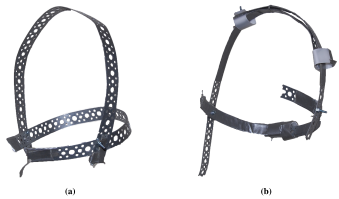
\includegraphics[height=6.5cm]{fig/prototype1.jpg}}\qquad\qquad
  \subfloat[]{\label{fig:prototype2}\includegraphics[height=6.5cm]{fig/prototype2.jpg}}
  \caption[1. og 2. utkast av prototype]{F�rste~\subref{fig:prototype1}
    og andre~\subref{fig:prototype2} utkast av prototype for hodeb�ylen}
  \label{fig:prototype}
\end{figure}

Inspirasjon til videreutvikling ble hentet fra en Koss PortaPro-hodeb�yle, og
det ble funnet en m�te � justere hodeb�ylen p� (fig.~\ref{fig:prototype2}).
Kravet om � lage en justerbar prototype som kunne tilpasses hver enkelt bruker,
ble dermed oppfylt. Noe som f�rst ble ansett som en fordel for � holde
hodeb�ylen godt p� plass, viste seg etter hvert � v�re en ulempe, for med ett
b�nd som gikk over hodet, og ett som gikk bak hodet, ble det veldig
problematiskt � ta hodeb�ylen p� og av hodet. Det ble alts� nok en gang en
konflikt mellom kravene i produktspesifikasjonen og resultatet.

Etter flere fors�k med spikerb�nd, ble det konkludert med at det ikke var det
best egnet metallet, siden det var svakt og knakk ofte ved mye b�ying. Det ble
derfor behov for noe annet. Alternativet ble metallet som blir brukt for � rense
kloakkr�r. Fordelen med dette metallet er at det er veldig solid og meget
slitesterkt, og hvis en b�yer det i forkant, er det veldig stivt. Derfor er det
mulighet til � f� det veldig stramt imellom kinn og sensor.

Med det nye <<vidundermetallet>> kunne det lages en helt ny m�te � justere
hodeb�ylen p� ut ifra inspirasjonen fra Koss PortaPro. Dette er illustrert i
figur~\ref{fig:justeringsboks} og~\ref{fig:prototype3}. Hodeb�ylen ble laget med
tre b�nd p� hver side og koblet sammen med noen justeringsbokser p� toppen av
hodet. Det nye justeringssystemet fungerte mye bedre enn det vi hadde fra f�r.
Hodeb�ylen var justerbart til flere brukere; � sette det av og p� var
uproblematisk, og det var behagelig � ha p� seg. Men kravet om at det skulle
legges press p� sensorene mot kinnet, var fortsatt ikke oppfylt.

\begin{figure}[t]
  \centering
  \subfloat[]{\label{fig:justeringMedlokk}\includegraphics[height=3cm]{fig/justeringMedLokk.png}}\qquad\qquad
  \subfloat[]{\label{fig:justeringUtenTopp}{\includegraphics[height=3cm]{fig/justeringUtenTopp.jpg}}}
  \caption[Justeringsboks]{Justeringsboks med lokk~\subref{fig:justeringMedlokk}
    og uten lokk~\subref{fig:justeringUtenTopp}.}
  \label{fig:justeringsboks}
\end{figure}

\begin{figure}[b]
  \centering
  \includegraphics[height=5cm]{fig/heleGreia.jpg}
  \caption[Tegning av 3. prototype]{Tegning av hodeb�ylens
    justeringsmuligheter}
  \label{fig:prototype3}
\end{figure}

Siden det hadde blitt bestemt at det ikke skulle v�re noe bak hodet for �
stramme opp, pga. praktiske �rsaker, kom vi frem til at det m�tte legges et
tykkere lag med metall litt lengre frem, som ble festet til det punktet som
sensorene p� hodeb�ylen skulle festes. Ved hjelp av dette oppfyltes alle kravene
som hadde blitt satt. Det eneste som manglet n� var � plassere sensorene og f�
det hele koblet til kretskortet med mikroprosessoren. (Mer om
sensorkonfigurasjon i kapittel~\ref{sec:funksjonalitet}.)

Det � f� festet sensorene p� hodeb�ylen ble gjort veldig enkelt: F�rst ble det
brukt to metallplater, en p� hver side. Deretter ble de sm� kretskortene som
sensorene er koblet sammen p�, festet p� metallplatene.

Det som n� ble vurdert, var om kretskortet som inneholder mikroprosessoren,
skulle plasseres p� hodeb�ylen. Siden det i utgangspunktet skulle v�re minst
mulig p� hodeb�ylen -- b�de fordi at det skulle v�re s� lett som mulig, og at
det ikke skulle bli mye elektronikk som en m� ta hensyn til n�r en skal plassere
hodeb�ylen p� brukeren -- m�tte det finnes et annet alternativ. Det ble
anskaffet en st�rre kabel med flere ledere i som ble festet p� toppen av
hodeb�ylen og koblet til sensorene p� hver sin side, slik at alle signalene fra
sensorene blir sendt samlet gjennom en kabel til prosessoren som skal ta imot.
P� enden av kabelen ble det montert et motstykke til en COM-port, dette for �
gj�re det enkelt � koble hodeb�ylen til �X-box�-en i kapittel~\ref{sec:xbox}
(fig.~\ref{fig:signalkabel}).

\begin{figure}[t]
  \centering
  \includegraphics[width=0.7\linewidth]{fig/overgangtilCOM.jpg}
  \caption[Signalkabel]{Bilde av signalkabel}
  \label{fig:signalkabel}
\end{figure}

\section{Resultat} % bilde-shait og -shit

En prototype av en hodeb�yle som oppfylte de kravene som hadde blitt satt i
forkant(figur~\ref{fig:ferdigprototype}). Det passer til flere brukere ved hjelp
av justeringsmulighetene, og det er lett � koble opp og komme igang med. Det er
to ulemper med den ferdige prototypen. Den ene er at justeringsdelen er litt
hard. Den andre er at hodeb�ylen ikke har nok press mot kinnet hvor sensorene
ligger. (Begge disse problemene vil v�re enkelt � l�se p� en ev. ferdig versjon
ved hjelp av noen som har en bedre bakgrunn i mekanikk og ev. annet utstyr som
gruppen ikke hadde til r�dighet.)

\begin{figure}[h]
  \centering
  \includegraphics[height=15cm]{fig/prototype3.jpg}
  \caption{Ferdig prototype}
  \label{fig:ferdigprototype}
\end{figure}


\cleardoublepage

\chapter[X-box (Uthus)]{X-box}
\label{sec:xbox}

\begin{figure}[h]
  \centering \fbox{\includegraphics[width=0.8\linewidth]{fig/x-boxsalangt.png}}
  \caption[Skisse av <<X-box>>]{Skisse av <<X-box>>, laget i AutoCAD}
  \label{fig:xboxACad}
\end{figure}

\begin{quote}\it
  \textbf{Sammendrag:} Inneholder en kort beskrivelse av hvordan <<X-box>>-en
  ble laget og hva den brukes til. Bakgrunnen til at <<X-box>>-en ble laget er
  gitt i kapittel~\ref{sec:hodeboyle}. <<X-box>>-en skal inneholde elektronikken
  som behandler dataen fra hodeb�ylen, og sender den videre til PC-en.
\end{quote}

\section{Problemstilling}

Det var et behov for et mellomledd mellom selve musen (hodeb�ylen,
kap.~\ref{sec:hodeboyle}) og datamaskinen. Dette bindingspunktet m�tte enkelt
kunne kobles til hodeb�ylen via COM-port og samtidig kunne kobles videre via USB
til PC-en. Det m�tte inneholde kretskortet til mikroprosessoren.

\section{Gjennomf�ring}

Prosjektgruppen fant ut at det skulle lages en boks som skulle ha to kontakter:
En COM-port som skulle kobles til hodeb�ylen, den andre kontakten skulle v�re
USB for � kommunisere videre inn til datamaskinen. Inne i boksen skulle det ogs�
v�re plass til kretskortet, samt til � sette p� testutstyr for � resette/justere
koden underveis. Det ble brukt en metalplate som b�ydes 90\degree\ p� hver side.
Dette utgjorde underlaget til boksen og 2 <<vegger>>. Kretskortet ble festet
inne i boksen ved hjelp av gaffateip, og plasseringen av kortet var s� n�r den
ene kanten uten <<vegg>> slik at den lett kan kobles til USB-kabelen (som en kan
se p� fig.~\ref{fig:xboxtopp}). Siden det skulle v�re COM-kontakt mot
hodeb�ylen, ble det laget et hull i den ene siden hvor COM-porten ble satt inn.
Det ble strukket ledninger som p� den ene siden var loddet fast til kretskortet,
den andre enden til COM-porten. N� var det alts� bare � koble i headsettet p�
den ene siden, og maskinen med USB p� den andre. <<That's Plug `n' Play!>>

\begin{figure}[h]
  \centering
  \includegraphics[width=0.6\linewidth]{fig/x-box2.jpg}
  \caption{Bilde av <<X-box>> fra toppen}
  \label{fig:xboxtopp}
\end{figure}

\section{Resultat}

En boks som skal v�re et bindeledd mellom PC-en og musen
(figur~\ref{fig:xboxferdig}. Den har en COM-port som var gruppens l�sning for �
p� en enkel m�te koble til hodeb�ylen. Videre g�r data fra hodeb�ylen inn til
kretskortet, og videre til maskinen som utf�rer �nskede operasjoner.

\begin{figure}[h]
  \centering
  \includegraphics[width=0.6\linewidth]{fig/x-box1.jpg}
  \caption{Bilde av ferdig <<X-box>>}
  \label{fig:xboxferdig}
\end{figure}


\cleardoublepage

\chapter[Elektronikk (Rishaug og Solem)]{Elektronikk} % hardware
\label{sec:elektronikk}

\begin{quote}\it
  \textbf{Sammendrag:} Dette kapittelet tar for seg valg av krets for tolking og
  digitalisering av sensordata og begrunnelse for valget. Det omhandler ogs�
  litt om den innebygde spenningsregulatoren som bruker str�m fra USB eller
  batteri. Kapittelet avrundes med en begrunnelse for valg av
  PC-grensesnitt. AT90USBkey har de funksjonene vi lette etter. Den kommuniserer
  og f�r str�m via USB-porten, og har en innebygd spenningsregulator som blir
  brukt til forspenning av de trykkf�lsome motstandene.
\end{quote}

\section{Problemstilling}

Det skal lages en krets for kommunikasjon med PC og Microsoft Windows.
Prosjektgruppen fokuserer p� de to grensesnittene Bluetooth og USB. Bluetooth er
et tr�dl�st grensesnitt som de fleste moderne PC-er enten allerede har mottager
for eller mulighet for � installere. USB er det mest brukte grensesnittet mot PC
i dag. Det er ogs� standard grensesnitt for PC-mus.

Det skal tas stilling til hvor behandlingen av data skal foreg�. Skal data
behandles i et bakgrunnsprogram p� Microsoft Windows, eller skal all
prosessering av data foreg� f�r oversending til PC?

Kretsen skal ikke sette krav til brukerens tekniske kunnskaper. Kretsen m� kunne
lese analoge data og digitalisere den � sende den videre
(analog-til-digital-omformer, ADC). Den skal ogs� v�re den billigste mulige
l�sningen som kan tilfredsstille alle spesifikasjonene p�
side~\pageref{sec:produktspes}.

\section{Valg av krets}

Prosjektgruppen velger � bruke AT90USBKey, som er en demokrets fra
Atmel~\cite{usbkey}.\footnote{\url{http://www.atmel.com/dyn/products/tools_card.asp?tool_id=3879}.}
Kretsen inneholder mikrokontrolleren AT90USB1287~\cite{uk}.

Denne kretsen ble valgt p� grunnlag av at den inneholder USB-brukergrensesnitt
mot PC, og er tidsbesparende siden prosjektgruppen slipper � designe en egen
krets. Mikrokontrolleren har en krystall p� 8~MHz og 128~kB minne. Den har ogs�
en �tte-ports ADC.

Siden kretsen er ment som en demonstrasjonskrets, bruker den to av ADC-portene
til temperaturavlesning (PF0 og PF3). Dette er ikke et problem for prototypen,
som bare bruker seks ADC-porter. Men �nsker man � bruke portene PF0 og PF3, kan
kretsen endres ved � fysisk fjerne tilkoblingen til temperaturavlesningen.

\begin{figure}[htb]
  \centering
  \includegraphics[width=0.6\linewidth]{fig/USBkey.png}
  \caption{AT90USBKey}
  \label{fig:AT90USBkey}
\end{figure}

Atmel har laget et USB Human Interface Device (HID)-kompatibelt musegrensesnitt
for mikrokontrolleren.\footnote{Lisensen for den medf�lgende programvaren til
  Atmel er gitt i \texttt{LICENSE.TXT} i \cite{program}.} Ved � bruke dette
sparer prosjektgruppen ytterligere med arbeidstid, men dette betyr at avlest
data m� behandles av mikrokontrolleren f�r den sendes til PC (for
databehandling, se kapittel~\ref{sec:funksjonalitet}).

Alternativet til denne kretsen var � designe en egen krets med
Bluetooth/USB-grensesnitt mot PC for bruker, og et programmeringsgrensesnitt for
utvikling. Denne kretsen ville ogs� blitt bygd rundt en mikrokontroller fra
Atmel, grunnet faglig kompetanse hos HiST. Mer om hva som kan gj�res videre er
gitt i kapittel~\ref{sec:veienvidere} -- design av kretsen(e) er utenfor
prosjektgruppens hovedproblemstilling (s.~\pageref{sec:hovedproblemstilling}).

\section{Str�mforsyning}
\label{sec:stromforsyning}

Den innebygde spenningskretsen p� AT90USBKey gj�r det mulig � bruke str�m
direkte fra USB-porten eller fra et eksternt batteri (se
kapittel~\ref{sec:veienvidere} for bruk av batteri). I v�rt tilfelle bruker vi
5~V spenningen fra USB-kontakten for � forsyne kretsen. Se
figur~\ref{fig:powerkrets-USB} for skjemategning over str�mforsyningen fra USB.
Fordelene med dette er at kretsen blir billigere og mindre komplisert.
Spenningen blir gjort om til ca. 3,3~V ved hjelp av en line�r
CMOS-spenningsregulator. Den n�yaktige utspenningen fra denne kan beregnes fra
formelen
\begin{equation}
  V_{CC3} = 1,25 \cdot \left(1 + \frac{R_{15}+R_{18}}{R_{19}}\right)
\end{equation}
Dette gir en utspenning p� $V_{CC3} = 3,266$~V. Denne spenningen blir ogs�
benyttet av sensorene som er koblet til.

\begin{figure}[htb]
  \centering
  \includegraphics[width=0.8\linewidth]{fig/power.png}
  \caption{AT90USBKey-powerkrets}
  \label{fig:powerkrets-USB}
\end{figure}

\section{USB-grensesnitt}

USB-teknologien har mange fordeler fremfor f.eks. PS2, RS232, LPT1 mfl. Siden
USB er det mest brukte PC-grensesnittet i dag, er alle nye datamaskiner og
maskiner fra tilbake til begynnelsen av 2000-tallet utrustet og klargjort for
dette. Enheter kan bli koblet til og fra uten � m�tte restarte systemet. Drivere
blir automatisk lastet inn og enheten blir dermed gjenkjent og gjort klar til
bruk (<<Plug `n' Play>>). En USB-inngang kan tilkobles s� mange som 127 enheter
og kan levere totalt opp til en halv ampere str�m til
periferiutstyr.\footnote{Standard 100~mA, maksimalt 500~mA etter foresp�rsel.}


\cleardoublepage

\chapter[Funksjonalitet (Solem og �ye)]{Funksjonalitet} % programvare
\label{sec:funksjonalitet}

\begin{quote}\it
  \textbf{Sammendrag:} Sensorene plasseres utenp� kinnene, to store
  knappsensorer og fire sm� bevegelsessensorer. Avlesningen av sensorverdiene er
  selvkalibrerende, og kan ogs� kalibreres manuelt. I utgangspunktet m�tte man
  presse kontinuerlig p� bevegelsessensorene for � flytte pekeren, men dette
  gjorde tungemuskelen fort sliten. P� bakgrunn av dette er sensorplasseringen
  justert lengst mulig frem p� kinnet, og <<ett-trykk-funksjonalitet>> gj�r det
  mulig � styre pekeren med lette trykk. Scroll og mulighet for � <<dra>>
  pekeren realiseres gjennom moduser, som aktiveres og deaktiveres ved � presse
  p� knappsensorene.
\end{quote}

\section{Problemstilling}

Plug `n' Play USB-musegrensesnittet mot PC, valgt i
kapittel~\ref{sec:elektronikk}, begrenser funksjonaliteten til \emph{standard
  musefunksjoner}: horisontal, vertikal og diagonal bevegelse, venstre- og h�yre
museknapp, og scroll.\footnote{Se produktspesifikasjonen,
  s.~\pageref{sec:produktspes}.} Den videre problemstillingen er hvordan disse
funksjonene skal aktiveres ved � bruke sensorene.

Den fysiske plasseringen av sensorene m� v�re enkel og intuitiv.
Implementeringen av musefunksjonene m� gj�res p� bakgrunn av antall sensorer og
plassering.

Det m� ogs� tas stilling til hvordan hver enkelt sensor avleses. Avleste verdier
m� n�dvendigvis sammenlignes med et \emph{nullniv�} for � avgj�re om de er i
bruk. M�lingene i kapittel~\ref{sec:sensorkap} tilsier at dette nullniv�et b�r
oppdateres med jevne mellomrom -- mikrokontrolleren b�r ta h�yde for at
sensorene kan henge seg opp, og kalibrere deretter.

\section{Plassering av sensorene}

\begin{figure}
  \centering
  \subfloat[]{\label{fig:bevsensorlinje}\includegraphics[height=5cm]{fig/bevsensorlinje.pdf}}\qquad\qquad
  \subfloat[]{\label{fig:bevsensortrekant}{\includegraphics[height=5cm]{fig/bevsensortrekant.pdf}}}
  \caption[Tre bevegelsessensorer i linje og trekant]{Sensorplate med tre
    bevegelsessensorer i linje~\subref{fig:bevsensorlinje} og
    trekant~\subref{fig:bevsensortrekant}}
  \label{fig:trebevsensorer}
\end{figure}

For at tungen skal kunne ha noen innvirkning p� sensorene uten � v�re i direkte
kontakt, m� sensorene festes utenp� kinnet. Dermed unng�r man ogs� sp�rsm�l
rundt hygiene ved brukerbytte.

Sensorene kan festes p� kinnet p� flere m�ter. Det er valgt � bruke en hodeb�yle
(se kap.~\ref{sec:hodeboyle}) med plater som sensorene festes
p�.\footnote{Festemekanismen kan videreutvikles, se
  kapittel~\ref{sec:veienvidere}.} Platene m� ha riktig antall sensorer, som
igjen m� ha riktig plassering mellom hverandre for � gi en god brukerf�lelse.
For � gj�re det intuitivt, er knapp- og bevegelsessensorene plassert p� hvert
sitt kinn.

De \emph{fire hovedretningene} regner vi som oppover, nedover, til venstre og
til h�yre. Dersom \emph{diagonal bevegelse} (kombinasjoner av hovedretningene)
ogs� er et krav, m� det plasseres minst tre sensorer p�
<<bevegelseskinnet>>.\footnote{Man \emph{kan} klare seg med f�rre dersom man
  bruker ulikt trykk for ulike retninger, men kapittel~\ref{sec:sensorkap}
  antyder at dette blir vanskelig.} Disse m� kunne aktiveres samtidig, og det m�
tas hensyn til hvilken sensor som er mest aktiv.

Som vi ser av figur~\ref{fig:trebevsensorer}, krever minst �n av hovedretningene
at man trykker p� to av de tre sensorene samtidig. Dette blir veldig vanskelig �
skille fra diagonal bevegelse, og derfor forkaster vi disse konfigurasjonene.
\emph{Hovedretningene er viktigere enn diagonalretningene.} Ved � bruke fire
sensorer for bevegelse, f�r hver hovedretning sin egen sensor, og diagonal
bevegelse f�s ved � aktivere to sensorer samtidig. Det er dette oppsettet vi
bruker i v�r \emph{f�rste tiln�rming}.

\section{F�rste tiln�rming}
\label{sec:forstetilnerming}

\begin{figure}[p]
  \centering
  \subfloat[]{\label{fig:sensorknapperklikk1}\raisebox{1cm}{\includegraphics[height=4cm]{fig/sensorknapper1.pdf}}}\qquad
  \subfloat[]{\label{fig:sensorknapperbev1}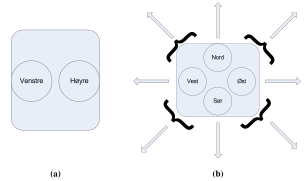
\includegraphics[height=6cm]{fig/bevsensorfirkant1.pdf}}
  \caption[Sensorplassering, f�rste tiln�rming]{F�rste tiln�rming: knapper p�
    venstre kinn~\subref{fig:sensorknapperklikk1} og bevegelse p� h�yre
    kinn~\subref{fig:sensorknapperbev1}}
  \label{fig:sensorknapper1}
\end{figure}

\noindent Den f�rste tiln�rmingen anvender fire \emph{sm�} sensorer
(type~FSR-400) for bevegelse p� venstre kinn og to \emph{store} sensorer
(type~FSR-402) for knapper p� h�yre kinn (fig.~\ref{fig:sensorknapper1}).
Bevegelsessensorene er plassert i <<stjerne>> og svarer til himmelretningene p�
et kompass -- ved � presse p� den �verste sensoren, g�r pekeren oppover, osv.
N�r trykket forsvinner, slutter bevegelsen.

\begin{figure}[p]
  \centering
  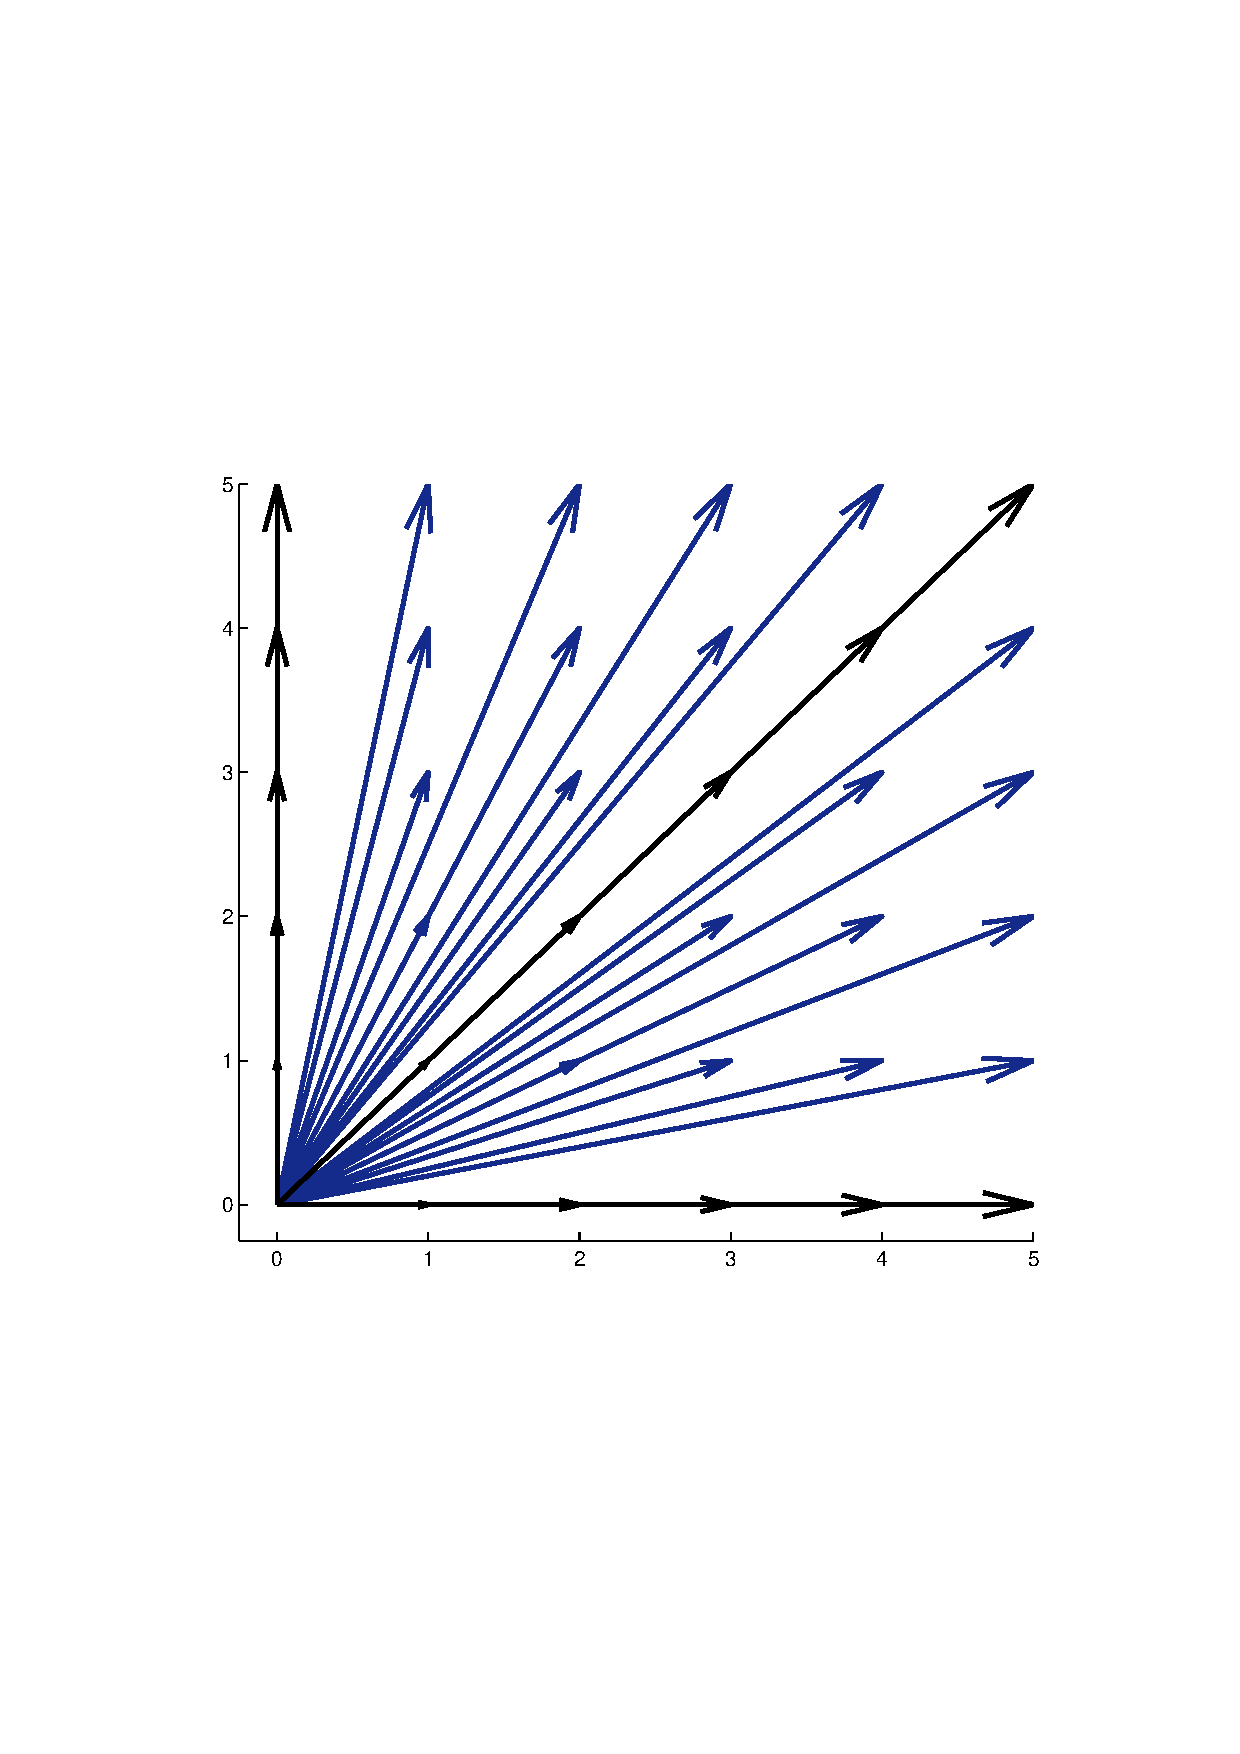
\includegraphics[height=5.5cm]{fig/retninger.pdf}
  \caption[Retninger i intervallet 0--90\degree]{Retninger i
    intervallet 0--90\degree.\\
    Tallene p� aksene ganges med basishastigheten.}
  \label{fig:retninger}
\end{figure}

Diagonal bevegelse f�s ved � trykke p� to n�rliggende sensorer samtidig. Dersom
man presser ekstra hardt, beveger pekeren seg opptil fem ganger raskere. Dette
gir teoretisk 72 flere retninger dersom man �ver ulikt trykk p� to n�rliggende
sensorer (fig.~\ref{fig:retninger}), dvs. en gjennomsnittlig oppl�sning p�
4,5\degree. (I praksis er bare de fire f�rste hastighetene oppn�elige, noe som
gir 40 ekstra retninger og 7,5\degree\ gjennomsnittlig oppl�sning.)

Knappsensorene er plassert side om side og svarer til henholdsvis venstre og
h�yre museknapp. Et enkelt trykk gir et enkelt klikk. For � dobbeltklikke, kan
man presse kontinuerlig slik at to klikk produseres i rask rekkef�lge.

Hvis en sensor kommer under u�nsket press, kan brukeren \emph{rekalibrere} den
ved � trykke p� motsatt kinn. Da tas den gjeldende sensorverdien som nullniv�,
og fremtidige sensorverdier sammenlignes med denne. Ellers kalibreres sensorene
automatisk n�r de ikke er i bruk.

\emph{Manglende funksjoner} er scroll og � <<dra>> musepekeren, dvs. holde
venstre museknapp inne mens pekeren beveges.

\subsection{Avlesning av �n sensor}

Hver sensor er forspent og koblet til en egen analog-til-digital-omformer (ADC)
som beskrevet i kapittel~\ref{sec:sensorkap}. ADC-ene avleses kontinuerlig --
opptil 125 ganger i sekundet -- og verdiene analyseres for � fastsl� om en
sensor er i bruk.

For � finne ut om en sensor er aktiv, m� den avleste verdien sammenlignes med en
verdi for n�r sensoren \emph{ikke} er i bruk, nullniv�et. Hvis den avleste
verdien er st�rre enn nullniv�et med en viss margin -- \emph{spranget} -- er
sensoren aktiv:
\begin{equation}
  \text{avlest verdi} > \text{nullniv�} + \text{sprang}
  \label{eq:sprang}
\end{equation}
N�r dette er oppfylt, sier vi at vi <<har et sprang>>. Marginen er fastsatt p�
forh�nd, og er litt st�rre for de store sensorene p� knappkinnet enn de sm�
sensorene p� bevegelseskinnet.

\begin{figure}
  \centering
  \includegraphics[height=10cm]{fig/kalibrering.pdf}
  \caption{Selvkalibrering og avlesning av sensor}
  \label{fig:kalibrering}
\end{figure}

Ideelt sett er nullniv�et 0~V. Men det er alltid en fare for at en av sensorene
kommer i klem, og dermed gir en h�yere verdi. Derfor b�r ikke nullniv�et
fastsettes p� forh�nd, men i stedet \emph{kalibreres} automatisk med
utgangspunkt i de avleste verdiene.

Figur~\ref{fig:kalibrering} viser avlesing og kalibrering av �n enkelt sensor.
Den f�rste avlesningen av sensoren etablerer nullniv�et, som videre avlesninger
sammenlignes med. Deretter avleses sensoren kontinuerlig og sammenlignes med
nullniv�et. Hvis differansen er stor nok, betraktes sensoren som aktiv, og en
musefunksjon utf�res. Hvis differansen ikke er stor nok, derimot, blir
nullniv�et \emph{rekalibrert}: nullniv�et settes til den avleste verdien.

Rekalibreringen begrenset til hver 250. gjennomgang i programmet~\cite{program},
slik at bare 250 p�f�lgende avlesninger uten <<sprang>> gir rekalibrering. Dette
medf�rer at dersom sensoren gradvis kommer under press (eller presset gradvis
opph�rer), vil nullniv�et oppdateres, mens hvis sensoren plutselig tas i bruk,
vil en musefunksjon utf�res.

Det kan tenkes at en sensor plutselig kommer under varig press selv om den ikke
er i bruk, f.eks. ved � flytte p� hodeb�ylen. I slike tilfeller kan det v�re
n�dvendig � kalibrere manuelt, noe som gj�res ved � aktivere en sensor p�
motsatt kinn. Hvis begge kinnene er <<aktive>>, sett fra programmets synspunkt,
settes nullniv�et p� nytt.

\subsection{Avlesning av flere sensorer}

Programmet lagrer de siste avleste verdiene til de seks sensorene i �n tabell,
og de seks nullniv�ene, som disse sammenlignes med, i en annen. Det g�r s�
igjennom tabellene parvis og sjekker dem opp mot ligning~(\ref{eq:sprang}) -- p�
leting etter en aktiv sensor.

\begin{figure}[p]
  \centering
  \subfloat[]{\label{fig:sensortabenkel}\includegraphics[width=0.7\linewidth]{fig/sensortabenkel.pdf}}

  \subfloat[]{\label{fig:sensortabtung}\includegraphics[width=0.7\linewidth]{fig/sensortabtung.pdf}}
  \caption[Avlesningsl�kker, enkel og avansert]{Avlesningsl�kker:
    enkel~\subref{fig:sensortabenkel} og avansert~\subref{fig:sensortabtung}}
  \label{fig:sensortab}
\end{figure}

N�r en aktiv sensor er funnet, er det to muligheter (fig.~\ref{fig:sensortab}).
Skal \subref{fig:sensortabenkel} resten av sensorene ogs� unders�kes, eller
\subref{fig:sensortabtung} s�ket avsluttes og den aktive sensoren returneres?
Hvis vi bare returnerer den f�rste aktive sensoren, m� vi legge inn en ekstra
<<nabosjekk>> av n�rliggende sensorer for � oppdage om to bevegelsessensor
brukes samtidig (diagonal bevegelse).\footnote{Dette gj�res ved � sl� opp i en
  matrise som inneholder informasjon om hvilke sensorer som er i n�rheten av
  hverandre. Hvis sensoren for bevegelse oppover er i bruk, for eksempel, �nsker
  vi bare � unders�ke sensorene for bevegelse til venstre og h�yre, ikke
  sensoren for bevegelse nedover.} Hvis vi s�ker gjennom hele tabellen, derimot,
vil alle aktive sensorer gi musefunksjoner (noe som h�ndterer diagonal bevegelse
automatisk), men kan gi u�nskede eller ingen musebevegelse ved noen
sensorkombinasjoner.

Fordelen med � gj�re det p� den andre og mer <<tungvinte>> m�ten i
figur~\ref{fig:sensortabtung}, hvor vi stanser s�ket n�r en aktiv sensor er
funnet og sjekker om denne sensoren har en aktiv <<nabosensor>>, er er at den er
mer fleksibel. Det er lettere � <<gardere>> mot aktive sensorer p� begge kinn,
som er signalet for manuell rekalibrering. Dessuten kan funksjonen som
returnerer den f�rste aktive sensoren, lett skrives om til � returnere den
\emph{mest} aktive sensoren dersom det viser seg vesentlig � skille mellom flere
sensortrykk.\footnote{Dette gj�r vi i andre tiln�rming,
  s.~\pageref{sec:andretilnerming}.} I v�r f�rste tiln�rming returneres bare den
f�rste aktive sensoren, men forholdene ligger til rette for en omskrivning.

For � produsere ett klikk av gangen, er det bygd inn en forsinkelse som overser
aktive knappsensorer etter at de er funnet aktive f�rste gang. Dette forhindrer
hundrevis av klikk mens sensoren er i bruk. Forsinkelsen er innstilt slik at
brukeren kan dobbeltklikke ved � presse kontinuerlig.

\subsection{Dr�fting}
\label{sec:forstedrofting}

Tiln�rmingen er utf�rlig testet i kapittel~\ref{sec:testingmedtungen}. De
viktigste funnene er at tungemuskelen fort blir sliten av � kontinuerlig presse
p� sensorene, og at det er tyngre dess lengre bak p� kinnet man kommer. Med
venstre og h�yre knappsensor plassert side om side, kommer venstre knappsensor
langt bak p� kinnet (fig.~\ref{fig:sensorknapperklikk1}). Det samme gjelder
h�yre bevegelsessensor, som er plassert i <<stjerne>> med de andre
bevegelsessensorene (fig.~\ref{fig:sensorknapperbev1}).

Det er ogs� et problem at det ikke er mulig � <<dra>> musepekeren. Ettersom
tungen ikke kan presse p� begge kinnene samtidig, kan dette bare implementeres
ved � aktivere en egen \emph{modus} hvor museknappen holdes nede. St�tte for
moduser vil ogs� gj�re det mulig � implementere scroll.

I v�r \emph{andre tiln�rming} roterer vi sensorplasseringen slik at den blir mer
vertikal med hensyn til munnen, og vi skriver om programmet til � <<huske>> en
oppgave over flere sensoravlesninger. Resultatet er mer omfattende, men ogs� mer
komfortabelt.

\section{Andre tiln�rming}
\label{sec:andretilnerming}

\begin{figure}[b]
  \centering
  \subfloat[]{\label{fig:sensorknapperklikk2}\raisebox{1cm}{\includegraphics[height=4cm]{fig/sensorknapper2.pdf}}}\qquad\qquad
  \subfloat[]{\label{fig:sensorknapperbev2}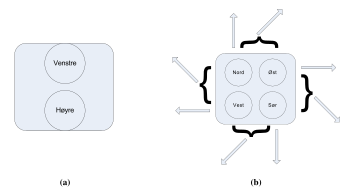
\includegraphics[height=6cm]{fig/bevsensorfirkant2.pdf}}
  \caption[Sensorplassering, andre tiln�rming]{Andre tiln�rming:
    knapper~\subref{fig:sensorknapperklikk2} og
    bevegelse~\subref{fig:sensorknapperbev2}.}
  \label{fig:sensorknapper2}
\end{figure}

\noindent I andre tiln�rming plasserer vi bevegelsessensorene i <<firkant>>
istedenfor <<stjerne>> for � f� dem lengre frem p� kinnet
(fig.~\ref{fig:sensorknapper2}). Knappsensorene er plassert ovenfor hverandre
istedenfor side om side.

Programmet tar n� utgangspunkt i den \emph{mest} aktive sensoren, ikke bare den
f�rste.

Sensorenes funksjoner avhenger av hvilken \emph{modus} programmet befinner seg
i. I utgangspunktet befinner programmet seg i \emph{normalmodus}, hvor
knappsensorene produserer klikk og bevegelsessensorene styrer pekeren. Den
viktigste forskjellen er m�ten pekeren styres p�.

\subsection{Normalmodus}
\label{sec:normmodus}

\begin{figure}
  \centering
  \subfloat[]{\label{fig:normalmodusstart}\includegraphics[width=\linewidth]{fig/normalmodusstart.pdf}}

  \subfloat[]{\label{fig:normalmodusbev}\includegraphics[width=\linewidth]{fig/normalmodusbev.pdf}}
  \caption[Normalmodus]{Normalmodus: klikk~\subref{fig:normalmodusstart} og
    bevegelse~\subref{fig:normalmodusbev}}
  \label{fig:normalmodus}
\end{figure}

Dette er programmets utgangspunkt (fig.~\ref{fig:normalmodus}). Hvis brukeren
trykker lett p� en knappsensor, produseres et klikk. Hvis brukeren trykker lett
p� en bevegelsessensor, beveger pekeren seg i sensorens retning, og
\emph{fortsetter � bevege seg} selv om brukeren ikke presser kontinuerlig.
Pekeren styres med lette trykk istedenfor kontinuerlig pressing, noe som er mer
behagelig for tungen.

N�r pekeren beveger seg, kan brukeren skifte retning ved � trykke p� en annen
bevegelsessensor, og f� bevegelsen til � opph�re ved � trykke p� samme sensor en
gang til. Pekeren beveger seg langsomt til � begynne med, for presisjonens
skyld, og s� raskere dersom brukeren ikke har skiftet retning etter et par
sekunder. Dette gj�r det lettere � bruke menyer og andre sm� omr�der p�
skjermen, uten at pekeren er like treg n�r den skal flyttes over st�rre omr�der.

Det er mulig � bevege pekeren enda raskere ved � presse kontinuerlig p� en
bevegelsessensor istedenfor � bruke <<ett-trykk-funksjonaliteten>>. Da vil
pekeren bevege seg raskere dess hardere man presser, og slutte � bevege seg n�r
trykket opph�rer, akkurat som i f�rste tiln�rming. Dette er praktisk for �
bevege seg over store deler av skjermen effektivt.

For presisjonens skyld er diagonal bevegelse \emph{deaktivert} n�r pekeren
beveges med lette trykk. Det er bare mulig � bevege seg diagonalt ved � presse
kontinuerlig p� sensorene.

\begin{figure}
  \centering
  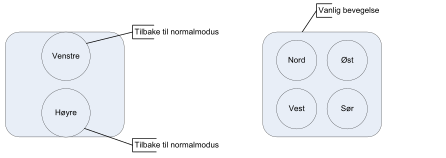
\includegraphics[width=0.85\linewidth]{fig/dramodus.pdf}
  \caption{<<Dra>>-modus}
  \label{fig:dramodus}
\end{figure}

\begin{figure}
  \centering
  \includegraphics[width=0.85\linewidth]{fig/scrollmodus.pdf}
  \caption{<<Scroll>>-modus}
  \label{fig:scrollmodus}
\end{figure}

\subsection{<<Dra>>-modus}

Ved � presse kontinuerlig p� knappsensorene istedenfor � bare trykke, bytter man
fra normalmodus til andre moduser. Venstre knappsensor bytter til <<dra>>-modus
(fig.~\ref{fig:dramodus}), slik at venstre museknapp holdes nede ogs� n�r
sensoren slippes. Dermed kan tungen flyttes over p� bevegelseskinnet for �
<<dra>> pekeren.

<<Dra>>-modus fungerer ellers som normalmodus; pekeren styres p� akkurat samme
m�te. For � g� tilbake til normalmodus, er det bare � ber�re knappsensoren en
gang til.

\subsection{<<Scroll>>-modus}

\noindent H�yre knappsensor bytter til <<scroll>>-modus
(fig.~\ref{fig:scrollmodus}). Man scroller oppover ved � presse p� �vre
bevegelsessensor, og nedover ved � presse p� nedre bevegelsessensor. For � g�
tilbake til normalmodus, trykker man p� en av knappsensorene.

\subsection{Dr�fting}
\label{sec:andredrofting}

Andre tiln�rming er utf�rlig testet i kapittel~\ref{sec:testingmedtungen}. Den
viktigste forskjellen fra f�rste tiln�rming er <<ett-trykk-funksjonaliteten>>,
som hindrer at tungen slites ut selv etter langvarig bruk. Den forbedrede
sensorplasseringen motvirker ogs� dette.

Presisjonen er betraktelig bedre takket v�re den langsommere pekerhastigheten
til � begynne med. Disse funksjonene kan kombineres: Ved � trykke fort to
ganger, kan man bevege pekeren i sm�, presise <<steg>>, f.eks. fra ett
menyelement til et annet.

<<Ett-trykk-funksjonaliteten>> gj�r det dessuten mulig � snakke mens man bruker
musen.

H�yere presisjon er viktig n�r man har behov for � <<dra>> pekeren, f.eks. for �
flytte vinduer. � innf�re moduser for slik funksjonalitet hever brukerterskelen,
men det viser seg enkelt � aktivere og deaktivere <<dra>>- og
<<scroll>>-modusene. Scrolling er en stor fordel n�r man surfer p� nettet, samt
i alle sammenhenger hvor man har behov for � rulle tekst. Disse to modusene gj�r
funksjonaliteten komplett.

Den st�rste utfordringen er � l�re opp tungen til � huske sensorenes plassering
p� kinnet. Dette blir bedre over tid, men krever litt t�lmodighet og innsats.


\cleardoublepage

\chapter[Testing med tungen (Rishaug og Solem)]{Testing med tungen}
\label{sec:testingmedtungen}

\begin{quote}\it
  \textbf{Sammendrag:} Inneholder en grundig test -- med resultater -- av
  funksjonaliteten og brukervennlighet til de to tiln�rmingene i
  kapittel~\ref{sec:funksjonalitet}. Viser at andre tiln�rming er en god
  forbedring av den f�rste. Videre dr�fting er gitt i forrige kapittel,
  avsnitt~\ref{sec:forstedrofting} og \ref{sec:andredrofting}.
\end{quote}

\section{Problemstilling}

Det er et behov for � teste om datamusen kan brukes til en dagligdags data�kt.
Testen gjennomf�res etter endringer i programmet som p�virker
brukerfunksjonaliteten. Testen brukes ogs� for � finne optimal plassering av
sensorene p� sensorplatene.

\section{Tester}

N�r man skal bruke en datamus, har man enkelte krav. Den skal v�re lett � styre,
og den skal v�re n�yaktig. En �kt frran datamaskinen tar gjerne litt tid, s�
hvor lenge kan man sitte f�r tungen blir sliten? Hvor god f�lelse av kontroll
oppn�r brukeren -- oppleves frustrasjon over datamusen under bruk? For � kunne
teste dette, er det laget noen enkle tester med stigende
vanskelighetsgrad.\\

\noindent\textbf{Metode:}
\begin{enumerate}
\item \textbf{�pne en snarvei fra skrivebordet:} velg en snarvei, f�r
  musepekeren over den og dobbeltklikk/�pne.
\item \textbf{�pne en snarvei fra startmenyen:} �pne <<Start>>-menyen og
  <<Programmer>>. �pne n� en forh�ndsbestemt snarvei fra denne menyen.
\item \textbf{Bruke nettleseren:} �pne Mozilla, g� til en avisside fra
  <<Favoritter>> eller hurtigmeny (f.eks. \url{http://www.vg.no/}), bla ned p�
  siden og �pne en artikkel.
\item \textbf{Bruk over tid:} �pne Microsoft Paint og pr�v � tegne en kopi av
  figur~\ref{fig:brukertest1}. Etter 15~minutter avsluttes testen, og resultatet
  sammenlignes med originalen. Er resultatet bra, og er tungen sliten? Utf�r
  testen to ganger for � se om det er en liten tilvenningskurve fra brukersiden.
\end{enumerate}
Testen er utf�rt med hodeb�ylen, men testeren har lagt ekstra trykk bak
sensorplatene med hendene. Med en bedre hodeb�yle vil dette v�re un�dvendig (se
kapittel~\ref{sec:veienvidere}).

\clearpage

\subsection{Resultater f�rste tiln�rming}

\begin{figure}[p]
  \centering
  \subfloat[]{\label{fig:brukertest1}\fbox{\includegraphics[width=0.5\linewidth]{fig/brukertest.png}}}

  \subfloat[]{\label{fig:brukertestresultat1a}\fbox{\includegraphics[width=0.5\linewidth]{fig/brukertestresultat1a.png}}}

  \caption[Tegnetest, f�rste tiln�rming]{Testtegning for bruk over tid \subref{fig:brukertest2},\\
    resultat i f�rste tiln�rming~\subref{fig:brukertestresultat2a}, f�rste og eneste fors�k}
  \label{fig:forstebrukertest}
\end{figure}

Se avsnitt~\ref{sec:forstetilnerming}, s.~\pageref{sec:forstetilnerming}, for
detaljer om f�rste tiln�rming.
\begin{enumerate}
\item \textbf{�pne en snarvei fra skrivebordet:} Musepekeren danser litt over
  skjermen, men med litt godvilje blir pekeren plassert over den forh�ndsvalgte
  snarveien (Papirkurven). Musebevegelsen g�r litt for fort, noe som gj�r det
  vanskelig � treffe ikonet. Det f�les ogs� litt tungt � holde sensoren inne for
  � bevege pekeren over skjermen. Holder venstre muspeker inne for �
  dobbeltklikke.
\item \textbf{�pne en snarvei fra startmenyen:} Merker at det krever mer
  presisjon og konsentrasjon � g� inn i <<Programmer>>-menyen. Musepekeren
  beveger seg litt for fort, noe som f�rer til at <<Start>>-meny-grenen til
  tider lukker seg. Det kommer frem at musen trenger en ny m�te � prioritere
  mellom sensoren(e) som er i bruk p�. Det hender musepekeren bytter retning
  uten at man vil det, og dette f�ltes ikke behagelig.
\item \textbf{Bruke nettleseren:} Velger � �pne nettsiden fra hurtigmenyen, blar
  nedover ved � trykke nederst p� rullefeltet. Det er noe vanskelig � treffe
  det, savner en scrollfunksjon. F�lelsen av kontroll over bevegelsen er ogs�
  her litt d�rlig, men knappene (h�yre/venstre) er lette � bruke. Litt tungt �
  bevege musepekeren rundt p� skjermen.
\item \textbf{Bruk over tid:} Ga opp etter syv minutter. Ble utrolig hemmet av
  at pekeren beveget seg for fort, og ble veldig sliten. Resultatet er gitt i
  figur~\ref{fig:brukertestresultat1a}.
\end{enumerate}
For dr�fting av resultatene, se avsnitt~\ref{sec:forstedrofting},
side~\pageref{sec:forstedrofting}.

\clearpage

\subsection{Resultater andre tiln�rming}

\begin{figure}[p]
  \centering
  \subfloat[]{\label{fig:brukertest2}\fbox{\includegraphics[width=0.5\linewidth]{fig/brukertest.png}}}

  \subfloat[]{\label{fig:brukertestresultat2a}\fbox{\includegraphics[width=0.5\linewidth]{fig/brukertestresultat2a.png}}}

  \subfloat[]{\label{fig:brukertestresultat2b}\fbox{\includegraphics[width=0.5\linewidth]{fig/brukertestresultat2b.png}}}

  \caption[Tegnetest, andre tiln�rming]{Testtegning for bruk over tid \subref{fig:brukertest2},\\
    resultat i andre tiln�rming f�rste fors�k~\subref{fig:brukertestresultat2a}, andre fors�k~\subref{fig:brukertestresultat2b}}
  \label{fig:andrebrukertest}
\end{figure}

Se avsnitt~\ref{sec:andretilnerming}, side~\pageref{sec:andretilnerming}, for
detaljer om andre tiln�rming.
\begin{enumerate}
\item \textbf{�pne en snarvei fra skrivebordet:} Litt vansker med � treffe rett
  sensor gj�r at pekeren til tider beveger seg feil vei. Trykker to ganger p�
  venstre musetast for � �pne den forh�ndsvalgte snarveien.
\item \textbf{�pne en snarvei fra startmenyen:} Bruker
  <<ett-trykk-funksjonaliteten>> for � bevege pekeren. Ingen problemer.
\item \textbf{Bruke nettleseren:} Glimrende. Gjorde speielt mye bruk av
  <<ett-trykk-funksjonaliteten>> og scrollfunksjonen, sv�rt behagelig i bruk.
\item \textbf{Bruk over tid:} Den delen av tegningen som krever h�yest
  presisjon, blomsten med blad og den dr�peformede figuren, er litt vanskelig.
  Men av fremskrittet fra figur~\ref{fig:brukertestresultat2a} til
  figur~\ref{fig:brukertestresultat2b} ser man at dette kan bli meget bra med
  litt �velse.
\end{enumerate}
For dr�fting av resultatene, se avsnitt~\ref{sec:andredrofting},
side~\pageref{sec:andredrofting}.


\cleardoublepage

\chapter[Prisestimering (Rishaug og Solem)]{Prisestimering}

\begin{quote}\it
  \textbf{Sammendrag:} Kapittelet inneholder en tiln�rming over prosjektets
  kostnad. Det er ogs� eksempler p� pris for egenproduksjon av krets.
  Prosjektets tiln�rmede utgifter er dr�yt 2000~NOK.
\end{quote}

\section{Utviklingskostnader}

Prosjektet er en bacheloroppgave p� HiST. Studentene f�r ikke l�nn under
arbeidet, s� utgiftene er konsentrert rundt materialkostnadene i
tabell~\ref{tab:utviklingskostnader}. Sensorene ble kj�pt inn av SINTEF, og
AT90USBKey ble kj�pt inn av HiST. Tabellen lister opp antatte kostnader for
disse. Prosjektets tiln�rmede utgifter er 1949~NOK i materialkostnader. Siden
dette er de eneste utgiftene, kan man konkludere med at prosjektet har v�rt
s�rdeles billig for oppdragsgiver.

Forslag til l�skomponenter best�r av en liste som inneholder overslag over
priser en eventuell egenproduksjon av kretsen vil koste. For 100~enheter vil de
l�se materialene til kretskortet tiln�rme en kostnad p� 13~518~NOK. Siden
kretsen ikke er designet, kan denne prisen avvike noe. Det er ikke laget noen
liste for materialpris til produksjon av hodeb�ylen. Det forventes at designen
og materialvalget p� denne m� utvikles videre (se
kapittel~\ref{sec:veienvidere}).

\clearpage

\begin{center}
  \footnotesize
  \begin{longtable}{lp{1.5cm}p{1.7cm}lll>{\raggedright\arraybackslash}p{1.5cm}}
    \caption{Materialkostnader uten frakt}\\
    \toprule
    Produktnavn   & Produsent            & Type                     & Antall & Enhetspris & Total pris        & Firma \\
                  &                      &                          &        & [NOK]      & [NOK]             &       \\
    \midrule
    AT90USBKey    & Atmel                & Demokrets\footnote{Tiln�rmede priser.} & 2 & 229 & 458             & Mouser electronics \\
    FSR-400       & Interlink            & Trykkf�lsom resistans*   & 25     & 23         & 575               & Interlink Electronics \\
    FSR-402       & Interlink            & Trykkf�lsom resistans*   & 25     & 26         & 650               & Interlink Electronics \\
    Veroboard     &                      & Koblingsbrett            & 1      & 59         & 59                & Clas Ohlson \\
    Teip          &                      & Gaffateip                & 1      & 79         & 79                & Clas Ohlson \\
    Metall 1      &                      & Stakepinne               & 7,6~m  & 39         & 39                & Jula \\
    Metall 2      &                      & Spikerb�nd $20 \times 1$~mm & 10~m & 89        & 89                & Clas Ohlson \\
                  &                      & Koblings\-enheter\footnote{Skruer/muttrer/ledninger og lignende.}  & 1 & -- & -- & HiST \\
    \midrule
    \multicolumn{7}{c}{Forslag til l�skomponenter} \\
    \midrule
    AT90USB1287   & Atmel                & Mikro\-kontroller        & 1      & 87         & 87                & Mouser electronics \\
    AT90USB1287   &                      &                          & 25     & 68         & 1700              & \\
    AT90USB1287   &                      &                          & 100    & 61,182     & 6118              & \\
    LP3982IMM-ADJ & National Semiconductor & Spennings\-regulator   & 10     & 14,65      & 146,5             & Arrow Electronics\\
    LP3982IMM-ADJ &                      &                          & 100    & 5,15       & 515               & \\
    LP3982IMM-ADJ &                      &                          & 1000   & 4,25       & 4250              & \\
    774-MXO45HS-3C-8.0  & CTS Electronic Components & Crystal Oscillators 8~MHz & 1 & 19,50 & 19,50           & Mouser electronics\\
	774-MXO45HS-3C-8.0  &                &                          & 100    & 15,24      & 1524              & \\
	774-MXO45HS-3C-8. 0 &                &                          & 1000   & 9,966      & 9996              & \\
	500075-1517   & Molex                & USB Mini-B vert          & 1	     & 51         & 51                & Mouser electronics\\
    500075-1517   &                      &                          & 100    & 29,43      & 2943              & \\
    500075-1517   &                      &                          & 1000   & 24,09      & 24090             & \\
	Motstander    &                      & Laveffekt-motstander*    & 1000   & 0,0594     & 59,4              & \\
	Kretskort     &                      & To-lags PCB*             & 100    & 21,4       & $2140 + 278$      & Microcirtec\\
	Kretskort     &                      & 	 			            & 1000   & 3,219      & $3219 + 730$      & \\
    \bottomrule\addlinespace
    \multicolumn{7}{l}{Tabellen benytter seg av omregningene \euro\ = 8,7 NOK og \$ = 6,6 NOK.}
    \label{tab:utviklingskostnader}
  \end{longtable}
\end{center}


\cleardoublepage

\chapter{Konklusjon}

Prototypen som er laget, kan utf�re alle standard musefunksjoner i Microsoft
Windows, s� vel som alle andre operativsystemer.

For kontrollering av musepekeren er det laget en <<ett-trykk-funksjonalitet>>,
som hindrer at tungen slites ut etter langvarig bruk. Brukeren starter en
bevegelse og stopper eller endrer retning ved �nsket plassering. Under denne
funksjonen beveger pekeren seg langsomt til � begynne med for � gi god
presisjon.

Man kan snakke mens man beveger musepekeren over skjermen, og det er mulig � be
venstre museknapp v�re aktiv mens man beveger musepekeren over skjermen. Det er
ogs� mulig � sette musen i en <<scroll>>-modus som gj�r surfing av nettsider og
lesing av dokumenter meget behagelig.

Den st�rste utfordringen er � l�re opp tungen til � huske sensorenes plassering
p� kinnet. Dette blir bedre over tid, men krever litt t�lmodighet og innsats.

De utdelte sensorene (FSR-400 og FSR-402) er veldig f�lsomme, men det kan v�re
vanskelig � f� utslag med tungen. Forskning p� hvordan sensorene er i kontakt
med kinnet kan forbedre dette.

Det ble laget en hodeb�yle for � gi riktig plassering av sensorene p� kinnet. P�
grunn av lite bakgrunnskunskap og utstyr, oppfyller ikke hodeb�ylen alle kravene
i produktspesifikasjonen. Sensorene er plassert utenp� kinnene -- to store
knappsensorer p� venstre og fire sm� bevegelsessensorer p� h�yre. Prototypen har
et problem med at sensorene ligger litt d�rlig mot kinnet.

Ved bruk av sensorene er det erfart at det m� v�re et godt press mot kinnet, og
de m� ligge lengst mulig fram mot munnen for at sensortypen skal kunne brukes i
et endelig produkt. Justeringsdelen er ogs� litt vanskelig, men designet har
potensial for videreutvikling.

Elektronikken som ble valgt for tolkning av sensordata, er demokretsen
AT90USBKey fra Atmel. Denne er basert p� mikrokontrolleren AT90USB1287 og
fungerte bra til utvikling av en prototype. Kretsen har innebygd �tte ADC-er,
hvorav seks blir benyttet til tolking av sensordata. Kretsen gj�r bruk av
USB-grensesnittet for overf�ring av data, s� vel som energitilf�rsel. Det er
integrert en spenningsregulator som benyttes til � forspenne sensorene. Denne er
sterk nok til � forsyne eventuelle tilleggskretser.

Det er laget en boks som omkapsler AT90USBKey (<<X-box>>), fordi demokretsen er
for stor til � festes p� hodeb�ylen.

Programkoden er skrevet for � v�re fleksibel ang�ende antall sensorer og portene
de kobles til, s� vel som valg av mikrokontroller. Teorien og m�lingene tilsier
at sensorene setter krav til en dynamisk verdi for hendelsesaktivering, og
kontinuerlig kalibrering. Dette problemet er l�st med programvare.

Programmeringsmessig er det lite som kan videreutvikles, ettersom programmet
implementerer alle funksjonene i HID-standarden. Flere funksjoner kan bare
implementeres p� toppen av det gjeldende grensesnittet, ved � skrive et program
eller driver p� PC-siden som h�ndterer signalene p� en egen m�te. Fordelen med �
begrense seg til HID-standarden er at musen ikke krever en egen driver og kan
dermed brukes overalt, ogs� p� Mac og Linux.

Utgiftene ved prosjektet var minimale, estimert til ca. 2000~NOK.\\

\noindent P� bakgrunn av rapporten, konkluderer prosjektgruppen med at det er
mulig � lage en tungestyrt musepeker som anvist. Det mekaniske og ergonomiske m�
imidlertid forbedres for � f� et salgbart produkt. % end


\cleardoublepage

\chapter{Veien videre}
\label{sec:veienvidere}

\begin{quote}\it
  \textbf{Sammendrag:} Inneholder en oversikt over hva prosjektgruppen mener kan
  vidreutvikles for enten � forbedre noe som allerede er implementert, eller
  forslag til hva som kan implementeres.
\end{quote}

\section{Hodeb�ylen}
\label{sec:vvidere_hodeboyle}

Hvis man designer et eget kretskort, kan kortets st�rrelse minskes betraktelig,
slik at det kan gj�res plass til det p� hodeb�ylen. Dette vil v�re mer praktisk
framfor � ha et mellomledd som <<X-box>> (s.~\pageref{sec:xbox}). Den eneste
kabelen fra hodeb�ylen vil da v�re USB-kabelen, som settes rett i PC-en. Denne
kabelen vil ogs� kunne tas helt av i andre enden. Det vil da v�re enklere �
sette hodeb�ylen p� bruker, og feste USB-kabelen etter at alt av utstyr er p�
plass.

Det neste vil v�re � forme platene brukt til justeringsboksen eller ev. hele
justeringsboksen. Det vil v�re �nskelig � kunne sette en <<styrke>> som skal til
for � justere hodeb�ylen ved behov. Slik som prototypen er n�, er justeringen
hard og ikke s� brukervennlig. Dette vil v�re noe som en person med litt
bakgrunnskunnskaper om mekanikk/design kan utf�re.

Det vil v�re en forbedring � skjule ledningene som g�r fra sensorene som er
plassert nede p� hver side. Disse er p� dagens prototype synlige, og veldig
s�rbare. Et lite rykk i en av disse kan f�re til at kabelen mister kontakt med
sensor, og musen vil v�re ubrukelig (noe som for~�vrig skjedde under det ene
m�tet mellom SINTEF og prosjektgruppen).

Det er ogs� et behov � se p� metallet som er brukt og alternativer til dette,
for � f� bedre trykk mot kinnet. Samme metall, men en tykkere utgave kan v�re en
god forbedring.

Sensorplatene til prototypen best�r av to kretskort som sensorene er teipet til.
Dette har vist seg lite slitesterkt, man b�r finne en alternativ l�sning. Det
kan v�re �nskelig for den enkelte bruker � rotere platene 180--360\degree, for
optimal brukervennlighet. Videre kan det hende at en buet eller fleksibel plate
kan fungere bedre som festepunkt til sensorene. Dette kan skape et mer n�yaktig
bilde av hvor tungen trykker, og en bedre brukeropplevelse. Det kan v�re
�nskelig med et <<mellomlegg>> mellom kinnet og sensorene for � kontrolere
treffpunktet.

\section{Elektronikk}
\label{sec:vvidere_krets}

Det vil v�re n�dvendig � designe en egen krets rundt
AT90USB1287-mikrokontrolleren for eventuell produksjon. N�r man f�rst er i gang
med dette, kan man se p� mulighetene for Bluetooth-implementering i tillegg til
USB. Ved � bruke et litium-batteri med laderkrets mot USB, kan produktet lades
n�r det ikke er i bruk, og det vil ikke v�re n�dvendig med batteribytte eller
ekstern lader. Om batteriet ikke f�r ladet lenge nok, b�r det v�re mulig � bruke
USB-grensesnittet.

\subsection{Bruk av batteri som str�mforsyning}
\label{sec:bbstrom}

Den innebygde spenningskretsen p� AT90USBKey gj�r at den kan forsynes med
batterispenninger mellom 8--15~V$_\text{DC}$. Ved normal bruk blir det m�lt at
kretsen trekker mellom 7,5--10~mA med et 9~V batteri tilkoblet. I tilegg kommer
Bluetooth-adapteren, som ogs� f�r spenningsforsyningen fra AT90USBKey. Ved
opperasjon vil denne �ke forbruket med 18,3~mA, slik at totalforbruket blir ca.
28~mA.

En oversikt over brukertid med ulike batterier tilkoblet kretsen er gitt i
tabell~\ref{tab:batteri}. Det er ogs� mulig � legge en funksjon inn i
programkoden som gj�r at Bluetooth-modulen g�r i hvilemodus ved inaktivitet.
Funksjoner som ikke er i bruk, vil sl�s av, og str�mforbruket vil falle
betraktelig.

Som man kan se av tabell~\ref{tab:batteri}, gir litiumbatterier overlegen
kapasitet fremfor standard NiMh-batterier (nikkel-metalhydrid). For � f� samme
kapasitet fra NiMh-batterier, vil vekten og st�rrelsen disse krever gj�re det
vanskelig � integrere kretsen p� hodeb�ylen. Ulempen med litiumbatterier er at
de krever en dedikert lader, og at de kan eksplodere ved
overoppheting/belastning.

En liten innebygd krets hindrer at batteriet blir utladet under en gitt
spenning, og ved ladning fungerer den samme kretsen slik at batteriet ikke skal
overlades. Uten denne ville batteriet ha blitt �delagt.

\subsection{Bluetooth}

For eventuell tr�dl�s dataoverf�ring kan det benyttes Bluetooth som
overf�ringsprotokoll. Dette vil f.eks. gj�re det enklere for brukeren � koble
seg til en annen datamaskin n�r dette f�rst er konfigurert. Datamaskinen vil da
automatisk kjenne igjen den virtuelle armen og vil av den kunne vekkes fra en
eventuell dvalemodus.

Teknologien benytter seg av radiofrekvensb�ndets 2,4~GHz-omr�de og har en
rekkevidde p� ca. 10~m. Overf�ringshastigheten ligger p� ca 1,0~Mb/s. Da det
benyttes radiob�lger, vil brukeren ikke hindres av at objekter i veien hindrer
signalet. For � �ke b�ndbredden og sikkerheten, benytter Bluetooth seg av
frekvens-hopping (Frequency Hopping Spread Spectrum, FHSS). Dette fungerer ved
at sender og mottager <<hopper>> fra frekvens til frekvens hele tiden etter et
bestemt m�nster, i frekvensomr�det 2,402~GHz til 2,480~Ghz~\cite{bluetooth}. En
ulempe ved bruk av denne teknologien som brukergrensesnitt, er at det kan oppst�
forsinkelse hvis datamaskinen belastes med parallelle oppgaver. Siden kretsen
ikke lenger vil v�re tilkoblet USB, m� den f� str�mtilf�rsel fra et batteri
eller annen ekstern str�mforsyning, som beskrevet i
kapittel~\ref{sec:elektronikk} og kapittel~\ref{sec:bbstrom}.

\vspace*{-0.5\baselineskip}
{\footnotesize
  \begin{longtable}[c]{llllll}
    \caption{Teoretisk operasjonstid med ulike batterityper}\\
    \toprule
    Batteritype        & Spenning      & Kapasitet & Belastningsstr�m & Operasjonstid & Vekt \\
                       & [V]           & [mAh]     & [mA]             & [h]           & [g] \\
    \midrule
    HR6F22 Ni-MH       & 8,4           & 200       & 30,0             & 6,7           & 39 \\
    6F22 Litium\footnote{Tilpasset lader m� anvendes for lading av litiumbatterier.} & 9,0 & 500 & 28,0 & 17,9 & 28 \\
    U9VLJ10 Litium*    & 9,0           & 1200      & 28,0             & 42,9          & 38 \\
    AAA Ni-MH 8x serie & $8 \times 1,2$ & 1000     & 26,3             & 38,0          & $8 \times 16$ \\
    AA Ni-MH 8x serie  & $8 \times 1,2$ & 2700     & 26,3             & 102,7         & $8 \times 30$ \\
    \bottomrule
    \label{tab:batteri}
  \end{longtable}}
\vspace*{-0.5\baselineskip}



\cleardoublepage

\appendix

\addcontentsline{toc}{chapter}{Bibliografi}
\begin{thebibliography}{99}
\bibitem[Bluetooth]{bluetooth}
  \url{http://www.bluetooth.com/Bluetooth/Technology/Works/}.

\bibitem[Vedlegg 1]{program}
  Programkode, dokumentert.

\bibitem[Vedlegg 2]{interlink}
  Datablad for Interlink sensorer.

\bibitem[Vedlegg 3]{usbkey}
  Datablad for AT90USBKey.

\bibitem[Vedlegg 4]{uk}
  Datablad for mikrokontrolleren.
\end{thebibliography}

\addcontentsline{toc}{chapter}{Bilag: CD}
\chapter*{Bilag: CD}
\label{sec:cd}

Vedlegg 1--4 foreligger p� CD, organisert som f�lger:

\section*{Vedlegg 1: Programkode}

\RaggedRight
Plassert i mappen \texttt{/Program}. Lisens for Atmel-kode har plasseringen
\texttt{/Program/at90usb128/demo/series6-hidmouse/LICENSE.txt}.

\section*{Vedlegg 2: Datablad for Interlink sensorer}

Plassert i mappen \texttt{/Datablader/Trykksensorer}.

\section*{Vedlegg 3: Datablad for AT90USBKey}

Plassert i mappen \texttt{/Datablader/Kretskort}.

\section*{Vedlegg 4: Datablad for mikrokontrolleren}

Plassert i mappen \texttt{/Datablader/Mikrokontroller}.

\cleardoublepage

\addcontentsline{toc}{chapter}{Figurer}
\listoffigures

\cleardoublepage

\addcontentsline{toc}{chapter}{Tabeller}
\listoftables

\end{document}
